\documentclass[a4 paper, 12 pt]{extarticle}
\usepackage{titlesec}
\titleformat{\section}{\normalfont\normalsize\bfseries}{\thesection}{1em}{}
\usepackage[utf8]{inputenc}
\usepackage[T2A]{fontenc}
\usepackage[russian]{babel}
\usepackage{amsfonts}
\usepackage{mathtext}
\usepackage{amsthm}
\usepackage{amsmath}
\usepackage{amssymb}
\usepackage{ragged2e}
\usepackage[unicode, pdftex]{hyperref}
\usepackage{upgreek}
\usepackage[left=3cm, right=1cm, top=1.5cm, bottom=2cm, bindingoffset=0cm]{geometry}
\usepackage{indentfirst}
\usepackage[pdftex]{graphicx}
\usepackage{enumerate}
\usepackage{tocloft}
\usepackage{textcomp}
\usepackage{setspace}
\graphicspath{{pictures/}}
\DeclareGraphicsExtensions{.pdf,.png,.jpg}
%\renewcommand{\thesection}{\arabic{section}.}

\renewcommand{\P}[1]{\mathbb{P} \left( #1 \right)}
\newcommand{\E}[1]{\mathbb{E} \left[ #1 \right]}
\newcommand{\R}{\mathbb{R}}
\newcommand{\tail}[1]{\overline{#1}}
\newcommand{\cip}{\overset{p}{\to}}
\newcommand{\Zi}{Z_{\infty}}
\setcounter{page}{1}



\newtheorem{lemma}{Лемма}[section]
\newtheorem{theorem}{Теорема}[section]
\newtheorem{remark}{Замечание}
\newtheorem{corollary}{Следствие}
\newtheorem{proposition}{Утверждение}[section]
\newtheorem{example}{Пример}
\newtheorem{Def}{Определение}[section]

\newcommand{\RomanNumeralCaps}[1]
{\MakeUppercase{\romannumeral #1}}

\doublespacing

\title{Задача рассеяния для уравнения Шрёдингера на метрических графах}
\author{С. А. Фадеев}
\date{\today}

\begin{document}
	\begin{singlespacing} % На титульнике одинарный интервал
		\thispagestyle{empty} % Не нумеруем титульный лист
		\begin{center}
			\normalsize{МИНИСТЕРСТВО НАУКИ И ВЫСШЕГО ОБРАЗОВАНИЯ РОССИЙСКОЙ ФЕДЕРАЦИИ}\\
			\hfill \break
			\normalsize{ФЕДЕРАЛЬНОЕ ГОСУДАРСТВЕННОЕ АВТОНОМНОЕ ОБРАЗОВАТЕЛЬНОЕ УЧРЕЖДЕНИЕ ВЫСШЕГО ОБРАЗОВАНИЯ}\\
			\hfill \break
			\normalsize{<<НОВОСИБИРСКИЙ НАЦИОНАЛЬНЫЙ ИССЛЕДОВАТЕЛЬСКИЙ ГОСУДАРСТВЕННЫЙ УНИВЕРСИТЕТ>>}
			\normalsize{(Новосибирский государственный университет, НГУ)}\\ 
			\hfill \break
			\large{\textbf{Механико-математический факультет}}\\
			\hfill\break
			\large{Кафедра теории функций}\\
			\hfill \break
			\large{Направление подготовки <<Математика>>, магистратура}\\
			\hfill\break
			\normalsize{\textbf{ВЫПУСКНАЯ КВАЛИФИКАЦИОННАЯ РАБОТА МАГИСТРА}}\\
			\hfill \break
			\large{Фадеева Степана Александровича}\\
			\hfill \break
			\large{\textbf{Задача рассеяния для уравнения Шрёдингера на метрических графах}}\\
			\hfill \break
		\end{center}
	\end{singlespacing}
	
	\noindent
	\begin{minipage}[t]{80mm}\parindent=0em
		\large{\textbf{<<К защите допущен>>}\par
			Заведующий кафедрой,\par
			д.ф.-м.н.,проф.\par
			\makebox[3cm]{\large{Медных А.Д.}}/\makebox[3cm]{\hrulefill}\par}
		\small{~(Фамилия, И.О.)~/~ ~(подпись, МП)}\par
		\large{«\makebox[1cm]{\hrulefill}»\makebox[4cm]{\hrulefill}2020 г.}
	\end{minipage}
	\hfill
	\begin{minipage}[t]{80mm}\parindent=1.4em
		\large{\textbf{<<Научный руководитель>>}\par
			к.ф.-м.н.\par
			с.н.с. ИМ им. Соболева\par
			\makebox[3cm]{\large{Дедок В.А.}}/\makebox[3cm]{\hrulefill}\par}
		\small{~(Фамилия, И.О.)~/~ ~(подпись, МП)}\par
		\large{«\makebox[1cm]{\hrulefill}»\makebox[4cm]{\hrulefill}2020 г.}
	\end{minipage}
	
	\hfill \break
	\begin{flushright}
		\large{Дата защиты:\large{<<\makebox[1cm]{\hrulefill}>>\makebox[4cm]{\hrulefill}2020 г.}}
	\end{flushright}
	
	\hfill \break
	\begin{singlespacing}
		\begin{center}
			\large{\textbf{\\Новосибирск,~2020}}
		\end{center} 
	\end{singlespacing}

	\section*{РЕФЕРАТ}
	{\it Название работы:} Задача рассеяния для уравнения Шрёдингера на метрических графах.
	
	{\it Количество страниц:} ??.
	
	{\it Количество используемых источников:} ??.
	
	{\it Ключевые слова}: задача рассеяния, уравнение Шрёдингера, метрические графы, компактные графы, законы Кирхгофа, квантовые графы, спектральная хирургия.
	
	Объект исследования --- рассеяние на метрических графах, прямые и обратные задачи. Цели дипломной работы ~--- исследование изменений данных рассеяния при топологических преобразованиях квантовых графов, а также изучение зависимости данных рассеяния от рассеивающих потенциалов. 	Исследование основано на технике спектральной хирургии квантовых графов, последовательном приближении рассеивающего потенциала ступенчатыми функциями, отслеживании изменения данных рассеяния при подобных приближениях. Область применения и рекомендации ~--- математическое моделирование мезоскопических систем, наноэлектроника, теория квантового хаоса, квантовые вычисления. В результате исследования были обобщены теоремы о спектральной хирургии квантовых графов, а также изучена сходимость данных рассеяния при константных возмущениях потенциала.
	
	\newpage
	\tableofcontents
	\newpage
	\section*{ВВЕДЕНИЕ}
	\addcontentsline{toc}{section}{ВВЕДЕНИЕ}
	Задача распространения волн в ветвящихся структурах и сетях играет важную роль во многих областях современной физики \cite{TransparentQuantumGraphs}. Для моделирования подобных явлений часто используются квантовые графы: компактные графы с добавленными бесконечными дугами. На каждой дуге определено одномерное стационарное уравнение Шрёдингера, в качестве граничных условий в узлах используются законы Кирхгофа для квантовых графов \cite{KirchhoffRule}. Важной особенностью рассматриваемых конструкций является распространение волн вдоль рёбер, сопровождающееся рассеянием (отражением)  волны в узлах графа. Бесконечно накапливаясь, отражённые волны могут оказать существенное влияние на решение задачи рассеяния.
	
	Впервые квантовые графы одномерных нитевидных структур, соединённых в вершинах, появились в работе H.~Kuhn \cite{Kuhn} и использовались для моделирования свободных электронов органических молекул. В данной работе органическая молекула была представлена набором атомов, расположенных в определённых координатах, соединённых связями, вдоль которых электроны подчиняются одномерному стационарному уравнению Шрёдингера с подходящим потенциалом.
	
	Позднее аналогичный подход был применён в задачах моделирования сверхпроводников  и искусственных материалов \cite{Superconductivity}, теории мезоскопических систем \cite{Kowal}, теории квантового хаоса \cite{QuantumChaos}.
	
	В настоящее время ведутся исследования в области спектральных оценок квантовых графов \cite{SpectralEstimates}, в том числе при использовании обобщённых граничных условий (delta couplings) \cite{deltaCouplings}. Кроме того, рассматриваются времязависимые модели в электромагнитных полях \cite{Popov1, Popov2}.
	
	Нас интересуют некомпактные графы, содержащие полубесконечные дуги. Такая гибкая конструкция позволяет воспроизводить черты многомерных объектов, будучи одномерной \cite{GerasimenkoPavlov}.
	
	В силу топологической сложности графов, в общем случае поиск решения задачи рассеяния является достаточно сложной проблемой. Методы решения, применяемые к одномерным и многомерным задачам рассеяния, не могут быть применимы к данной задаче. Поэтому для решения задачи рассеяния на топологически сложном графе предлагается найти решение на топологически примитивных графах, а затем склеить друг с другом примитивы согласно некоторым правилам преобразования данных рассеяния. Этот метод называется техникой спектральной хирургии квантовых графов и описан в \cite{SpectralSurgery}.
	
	Данная работа состоит из двух частей. 
	
	Первая часть посвящена обобщению теорем спектральной хирургии. Получен результат о склейке двух графов, содержащих неизвестную компактную часть, известные данные рассеяния. В дальнейшем планируется обобщить полученные результаты для получения теоремы о склейке по произвольному количеству дуг полубесконечной длины.
	
	Вторая часть посвящена исследованию зависимости данных рассеяния на некомпактном графе от рассеивающих потенциалов. В силу сложности задачи рассеяния, были рассмотрены некоторые частные случаи графов и потенциалов на внутренних дугах. Для данных частных случаев графов (петля и кольцо с полубесконечными дугами) были решены прямые задачи по определению данных рассеяния для различных потенциалов. Были исследованы свойства данных рассеяния на таких графах со ступенчатыми потенциалами на внутренних ребрах, численно изучены эффекты возникновения новых волн при трансформации потенциала. В дальнейшем планируется применить полученные результаты для построения вычислительно эффективного метода решения обратной задачи рассеяния.
	
	
	\newpage
	\section{ОДНОМЕРНАЯ ЗАДАЧА РАССЕЯНИЯ}
	\subsection{ОБЩИЕ СВЕДЕНИЯ}
	\addcontentsline{toc}{section}{ОБЩИЕ СВЕДЕНИЯ}
	В теории рассеяния на квантовых графах основным объектом исследования является одномерное стационарное уравнение Шрёдингера
   \begin{equation*}
   -\frac{\hbar^2}{2m}\frac{d^2\psi}{d x^2}+v\psi=E\psi,
   \end{equation*}
   Заменив $2E/\hbar^2=k^2$ и $2mv/\hbar^2=u$, получим уравнение в безразмерной форме
   \begin{equation}\label{Schred1D}
   -\frac{d^2\psi}{d x^2}+u\psi=k^2\psi.
   \end{equation}
   
   \begin{Def}
   	Оператор Шрёдингера ~--- это дифференциальный оператор \newline  $-\frac{d^2}{d x^2}+u$.
   \end{Def}

   \begin{Def}
   	Рассеивающий потенциал (потенциал оператора Шрёдингера) ~--- это коэффициент $u$.
   \end{Def}

   \begin{Def}
    Спектральный параметр ~--- это параметр $k$.
   \end{Def}
	Отметим, что при $k=0$, получаем описание движения частицы в отсутствие внешних полей
	\begin{equation*}
	\psi=c_1e^{ikx}+c_2e^{-ikx}, \quad \text{если} \quad u\equiv0.
	\end{equation*}
    Также будем называть волновой функцией решение уравнения Шрёдингера.
    
    Волновая функция обладает следующими свойствами \cite{Peisakhovich, Landau}:
    \begin{itemize}
    	\item $\psi\left(x\right)$ ~--- комплекснозначная функция
    	\item $\psi\left(x\right)$ ~--- конечная функция (интегрируема с квадратом)
    	\item $\psi\left(x\right)$ ~--- однозначная функция координат
    	\item $\psi\left(x\right)$ ~--- непрерывная функция
    \end{itemize}

   При этом физический смысл имеет только квадрат модуля волновой функции: \linebreak $\left|\psi\left(x\right)\right|^2 = \psi\left(x\right) \psi\left(x\right)^*$ ~--- плотность вероятности нахождения частицы в некоторой области.
   
   В теории рассеяния на квантовых графах часто налагают дополнительные ограничения на потенциалы: они считаются измеримыми функциями с конечными первыми моментами
   
   \begin{equation*}
   \int_{-\infty}^{\infty}(1+|x|)|u(x)|dx<\infty.
   \end{equation*}
   
   Это условие означает, что потенциал $u$
   достаточно быстро (быстрее чем $x^{-\delta}$, $\delta\geq2$)
   убывает при $|x|\rightarrow\pm\infty$.
   
   Переходя к асимптотике, получим:
   $$
   -\psi''=k^2\psi, \quad |x|\gg1,
   $$

   откуда имеем
   
   $$
   \psi=c_1e^{ikx}+c_2e^{-ikx}+o(1), \quad x\rightarrow\pm\infty.
   $$
   
   Без ограничений общности, будем считать, что источник волны находится в $+\infty$. Это соответствует следующему начальному условию на $-\infty$:
   \begin{equation}\label{SchredBorderMInf}
   \psi=e^{-ikx}+o(1), \quad x\rightarrow-\infty,
   \end{equation}
   Тогда асимптотический вид волновой функции на $+\infty$ имеет вид:
   \begin{equation}\label{SchredBorderPInf}
   \psi=a(k)e^{-ikx}+b(k)e^{ikx}+o(1), \quad
   x\rightarrow+\infty.
   \end{equation}
   
   \begin{Def}
   	Коэффициент прохождения ~--- это коэффициент $a = a\left(k\right)$, соответствует частице, движущейся влево.
   \end{Def}

   \begin{Def}
   	Коэффициент отражения ~--- это коэффициент $b = b\left(k\right)$, соответствует частице, движущейся вправо.
   \end{Def}

   \begin{Def}
   Данные рассеяния ~--- это набор всех коэффициентов отражения и прохождения.
   \end{Def}

   \begin{Def}
   	Прямая задача рассеяния ~--- вычисление данных рассеяния по заданному потенциалу согласно формулам (\ref{Schred1D}), (\ref{SchredBorderMInf}), (\ref{SchredBorderPInf}).
   \end{Def}

   \begin{Def}
   	Обратная задача рассеяния ~--- вычисление потенциала по заданным данным рассеяния согласно формулам (\ref{Schred1D}), (\ref{SchredBorderMInf}), (\ref{SchredBorderPInf}).
   \end{Def}

   В теории квантовых графов данные рассеяния обычно представляются в виде матрицы рассеяния. Так, для одномерного стационарного уравнения Шрёдингера она определяется асимптотиками:
   
   TODO: похоже, что тут надо поменять $s_{12} \leftrightarrow s_{11}, \quad s_{21} \leftrightarrow s_{22}$ .
   \begin{gather*}
   \begin{aligned}
   \psi_1(x,k)&=e^{ikx}+s_{12}(k)e^{-ikx}+o(1), \quad &x\rightarrow-\infty,\\
   \psi_1(x,k)&=s_{11}(k)e^{ikx}+o(1), \quad &x\rightarrow+\infty,\\
   \psi_2(x,k)&=e^{-ikx}+s_{21}(k)e^{ikx}+o(1), \quad &x\rightarrow+\infty,\\
   \psi_2(x,k)&=s_{22}(k)e^{-ikx}+o(1), \quad &x\rightarrow-\infty.
   \end{aligned}
   \end{gather*}
   

   \begin{Def}
   	$S$-матрица (матрица рассеяния) ~--- это матрица 
    \begin{equation}\label{DSM}
    S(k)=\left(%
    \begin{array}{cc}
    s_{11}(k) & s_{12}(k) \\
    s_{21}(k) & s_{22}(k) \\
    \end{array}%
    \right)
    \end{equation}
   \end{Def}

   Л.~Д.~Фаддеевым доказано \cite{SMatrix}, что существуют решения с заданными асимптотиками, а также $S$-матрица унитарна и удовлетворяет условию симметрии $s_{11}\left(k\right) = s_{22}\left(k\right)$.
   
   \subsection{КОНСТАНТНЫЙ ПОТЕНЦИАЛ}
   Предположим, что в уравнении (\ref{Schred1D}) потенциал $u$ измерим, имеет вид $$u = u\left(x\right) \equiv \tilde{u} = const \in \mathbb{R}$$ и обладает конечным первым моментом, тогда имеем линейное однородное дифференциальное уравнение второго порядка с постоянными коэффициентами. Его характеристическое уравнение имеет вид
   \[-\lambda^2+\tilde{u} = k^2\]
   и корни
   \[\lambda_{1,2}=\pm \sqrt{\tilde{u}-k^2}\]
   Тогда общее решение имеет вид
   \[
   \psi\left(x\right)= C_1 e^{\sqrt{\tilde{u}-k^2}x} + C_2 e^{-\sqrt{\tilde{u}-k^2}x}
   \]
   
   В частности, если $\tilde{u} \in \mathbb{R}, \ \tilde{u}-k^2<0$, то, обозначив $-a^2=\tilde{u}-k^2$, решение можно записать в виде \[\psi\left(x\right)= C_1 \cos\left(ax\right)+ C_2 \sin\left(ax\right)\].
   
   \section{ЗАДАЧА ШТУРМА-ЛИУВИЛЛЯ НА КОМПАКТНЫХ ГРАФАХ}

   Рассмотрим произвольный взвешенный граф с рёбрами конечной длины и семейство операторов $\{L_i\}_{i=1}^B$

   \begin{equation}\label{LOp}
   L_i = -\frac{d^2}{dx_i^2} + u_i(x_i).
   \end{equation}

   Каждому ребру $b$ сопоставим отрезок $[0, l_b]$, где $l_b$ --- длина ребра.
   Определим следующие пространства:
   \begin{gather*}
   D(L_i)={\varphi(x_i):\varphi\in C_0^\infty[0,l_i]},\\
   L_2(G)=\sum_{i=1}^{B}\oplus L_2[0, l_i],\\
   D(G)=\sum_{i=1}^{B}\oplus C_0^\infty[0,l_i],\qquad D(G)\subset L_2(G)
  \end{gather*}

  и оператор
  \begin{equation}\label{LG}
  L_G=\sum_{i=1}^{B}\oplus L_i.
  \end{equation}

  Поставим условия в вершинах графа следующим образом:

  \begin{enumerate}\label{Kirchoff}
	\item $\psi$ непрерывна в узлах графа,
	\item сумма производных волновой функции по всем дугам с учётом ориентации рёбер в каждой вершине равна нулю.
  \end{enumerate}

  Данные граничные условия называют законами Кирхгофа для квантовых графов \cite{KirchhoffRule}. Они имеют физический смысл: первое условие соответствует непрерывности волновой функции в вершине, второе условие соответствует сохранению потока в вершине.

Имеют место следующие теоремы \cite{GerasimenkoPavlov}:

   \begin{theorem}
	Дифференциальное выражение $L_G$ и граничные условия 1) и 2)
	определяют самосопряженный в $L_2(G)$ оператор.
   \end{theorem}

  \begin{theorem}
	Спектр оператора $L_{G}$ на компактном графе с локально измеримым
	потенциалом дискретен.
  \end{theorem}

  \begin{Def}
  	Задача Штурма-Лиувилля на компактном графе $G$ ~--- это задача поиска спектра оператора $L_{G}$.
  \end{Def}

  \begin{Def}
  	Волновая функция $\psi$ ~--- это $B$-компонентный вектор $$\psi=\left(\psi_{b_1}(x_{b_1}),
  	\psi_{b_2}(x_{b_2}),\ldots,\psi_{b_B}(x_{b_B})\right)^T,$$
  	
  	где множество $\left\{b_i\right\}_{i=1}^{B}$ состоит из различных
  	ребер графа $G$.
  \end{Def}

  На каждом ребре $b$ компонента волновой функции $\psi_b(x_b)$
  удовлетворяет одномерному стационарному уравнению Шрёдингера:

  \begin{equation}\label{Shred1}
   \left(-\frac{d^2}{dx_i^2} +
    u_i(x_i)\right)\psi_b(x_{i})=k^2\psi_b(x_{i})\qquad(b=[i,j]),
  \end{equation}

  а в каждой вершине -- граничным условиям 1) и 2). Заметим, что
  введённая ранее ориентация на рёбрах не является существенным
  требованием, и служит лишь для удобства вычисления производных по
  исходящим дугам.
  
  \pagebreak
  
  \section{ЗАДАЧА РАССЕЯНИЯ НА НЕКОМПАКТНЫХ ГРАФАХ}
  
  Рассмотрим произвольный некомпактный граф, который можно получить добавлением некоторого количества полубесконечных дуг к компактному графу.
  Аналогичным образом можно определить самосопряженный оператор
  $L_G$. Отличие состоит лишь в том, что некоторые операторы
  $\{L_i\}$ действуют в $L_2(0, \infty)$ и
  $D(L_i)=\{\varphi:\varphi\in C_0^\infty[0,\infty]\}$.
  
  \begin{gather*}
  L_2(G)=\sum_{B'}\oplus L_2[0, l_i]\bigoplus\sum_{B''}\oplus
  L_2[0,\infty],
  \\
  D(G)=\sum_{B'}\oplus C_0^\infty[0,l_i]\bigoplus\sum_{B''}\oplus
  C_0^\infty[0,\infty]
  \end{gather*}
  
  Исходя из нужд задачи рассеяния потенциалы $u_i$ на
  соответствующих ребрах будем считать вещественными измеримыми
  функциями с конечным первым моментом
  
  \begin{equation}
  \int_0^\infty(1+x_i)|u_i(x_i)|dx_i<\infty.
  \end{equation}
  
  Рассмотрим несколько примеров.
  
  \subsection{ЗАДАЧА РАССЕЯНИЯ НА ЗВЁЗДНОМ ГРАФЕ}
  Рассмотрим задачу рассеяния на графе-звезде, содержащем 3 дуги и 1 вершину, все потенциалы нулевые.
  \begin{figure}[!htb]
  	\centering
  	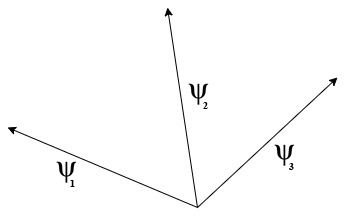
\includegraphics[scale=0.5]{star.jpg}
  \end{figure}
  Ищем решение в виде:
  \[\begin{split}
  \psi_1\left(x\right) &= C_1 e^{ikx} + C_2 e^{-ikx}, \\
  \psi_2\left(x\right) &= C_3 e^{ikx} + C_4 e^{-ikx}, \\
  \psi_3\left(x\right) &= C_5 e^{ikx} + C_6 e^{-ikx}.
  \end{split}\]
  
  Сопутствующая система имеет вид:
  \[\begin{cases}
  \psi_{1}\left(k,0\right)=\psi_2\left(k,0\right), \\
  \psi_{1}\left(k,0\right)=\psi_3\left(k,0\right), \\
  \psi_1^\prime\left(k,0\right)+\psi_2^\prime\left(k,0\right)+\psi_3^\prime\left(k,0\right)=0.
  \end{cases}
  \]
   Переписывая систему в терминах $C_1,C_2,C_3,C_4,C_5,C_6$, получим СЛАУ вида $Ac=b$ :
   \[ A = \left(\begin{smallmatrix}
   1 & -1 & 0 \\
   1 & 0 & -1 \\
   1 & 1 & 1
   \end{smallmatrix}\right), b = \left(\begin{smallmatrix}
   -1 \\
   -1 \\
   1
   \end{smallmatrix}\right), \ 
   \left(\begin{smallmatrix}
   1 \\
   0 \\
   1
   \end{smallmatrix}\right),
   \left(\begin{smallmatrix}
   0 \\
   1 \\
   1
   \end{smallmatrix}\right).\]
   
   Решая эту систему, получим искомую матрицу рассеяния:
   \begin{equation}
   \label{starData}
   S(k)=
   \begin{pmatrix}
   -1/3 & 2/3 & 2/3 \\
   2/3 & -1/3 & 2/3 \\
   2/3 & 2/3 & -1/3 
   \end{pmatrix}
   \end{equation}
   
   \subsection{ПЕТЛЯ С $n$ ПОЛУБЕСКОНЕЧНЫМИ ДУГАМИ}
   Рассмотрим граф,
   \begin{figure}[!htb]
   	\centering
   	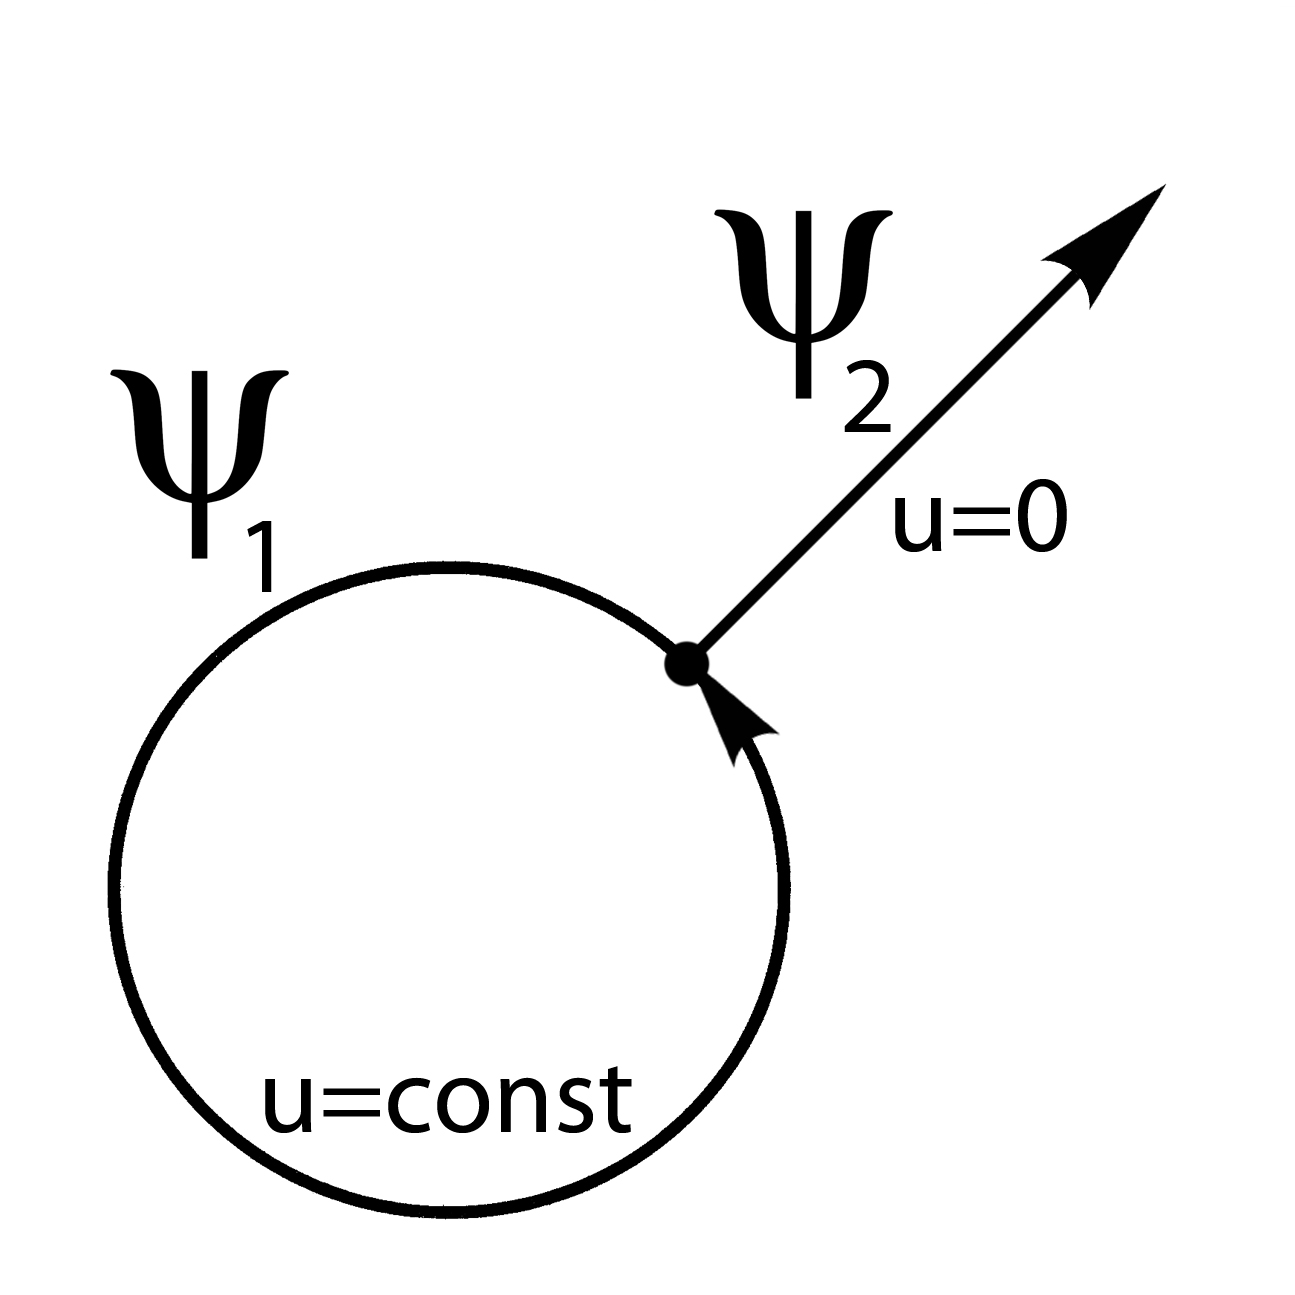
\includegraphics[scale=0.5]{one-arrow.jpg}
   \end{figure}
   \\состоящий из петли и одной полубесконечной дуги. Предположим, что на петле длины $a$ задан некоторый константный потенциал, а на полубесконечной дуге потенциал нулевой.
   Ищем решение в виде
   \[\psi\left(k\right) = \left\{\psi_1\left(k,x\right), \psi_2\left(k,x\right)\right\}, \ \text{где}\]
   \[
   \psi_1 = c_1\cdot e^{\sqrt{u-k^2} \cdot x} + c_2\cdot e^{-\sqrt{u-k^2} \cdot x}, \ x \in \left[0,a\right],\]
   \[\psi_2 = c_3 \cdot e^{ikx}+c_4 \cdot e^{-ikx}, \ x \in \left[0,+\infty\right)\]
   
   Сопутствующая система законов Кирхгофа имеет вид:
   \[\begin{cases}
   \psi_1\left(k,0\right)=\psi_1\left(k,a\right), \\
   \psi_{1}\left(k,0\right)=\psi_2\left(k,0\right), \\
   \psi_1^\prime\left(k,0\right)-\psi_1^\prime\left(k,a\right)+\psi_2^\prime\left(k,0\right)=0.
   \end{cases}
   \]
   Без ограничений общности, $c_3=R, \ c_4 = 1$. Это предположение соответствует ситуации, в которой волновой пакет единичной амплитуды попадает в граф из бесконечно удалённой точки по полубесконечной дуге, рассеивается на графе, а затем возвращается с некоторым коэффициентом $R$. Переписывая систему в терминах $c_1,c_2,R$, получим СЛАУ вида $Ac=b$:
   
   \[ A = \left(\begin{smallmatrix}
   1-e^{\sqrt{u-k^2}} & 1-e^{-\sqrt{u-k^2}} & 0 \\
   1 & 1 & -1 \\
   \sqrt{u-k^2}-\sqrt{u-k^2} \cdot e^{\sqrt{u-k^2}} & -\sqrt{u-k^2}+\sqrt{u-k^2} \cdot e^{\sqrt{u-k^2}} & ik
   \end{smallmatrix}\right)\]
   \[b = \left(\begin{smallmatrix}
   0 \\
   1 \\
   ik
   \end{smallmatrix}\right)
   \]
   Обозначив $p=\sqrt{u-k^2}$, получим формулу для коэффициента отражения:
   \begin{equation}
%   \label{OneDimensionalReflection}
   R\left(k,u\right) = {\frac { \left( ik+2\,p \right) {e}^{2\,pa}-ik-4\,p{e}^{pa}+2\,p}{ \left( ik-2\,p \right) {e}^{2\,pa}-ik+4\,p{e}^{pa}-2\,p}}
   \end{equation}
     
   Непосредственным вычислением можно убедиться, что 
   \begin{theorem}
   	$\left|R\left(k,u\right)\right| = 1$
   \end{theorem}
   
   В случае $n=1$ матрица рассеяния одномерна: $S = \left(R\left(k,u\right)\right)$. 
   В случае $n \geqslant 1$ матрица рассеяния имеет размер $(n-1) \cdot (n-1)$ (по количеству рёбер бесконечной длины).
   
   Физический смысл матрицы рассеяния понятен: в $i$-й строке на $i$-м месте находится коэффициент отражения $R_{ii}$, на $j$-м месте стоит коэффициент прохождения $T_{ij}$, $i \in \left\{1,\ldots,n-1\right\}, j \in \left\{1,\ldots,n-1\right\}\setminus i $.  Это соответствует ситуации, в которой волновой пакет единичной амплитуды попадает в граф из бесконечно удалённой точки по бесконечному ребру с номером $i$, рассеивается на графе, а затем возвращается с коэффициентом отражения $R_{ii}$ по ребру с номером $i$, с коэффициентами прохождения $T_{ij}$ по рёбрам с номерами $j \in \left\{1,\ldots,n-1\right\}\setminus i $.
   
   Для петли с $n$ полубесконечными рёбрами имеем СЛАУ $(n+1)\cdot (n+1)$ с матрицей:
   \begin{figure}
   	\centering
   	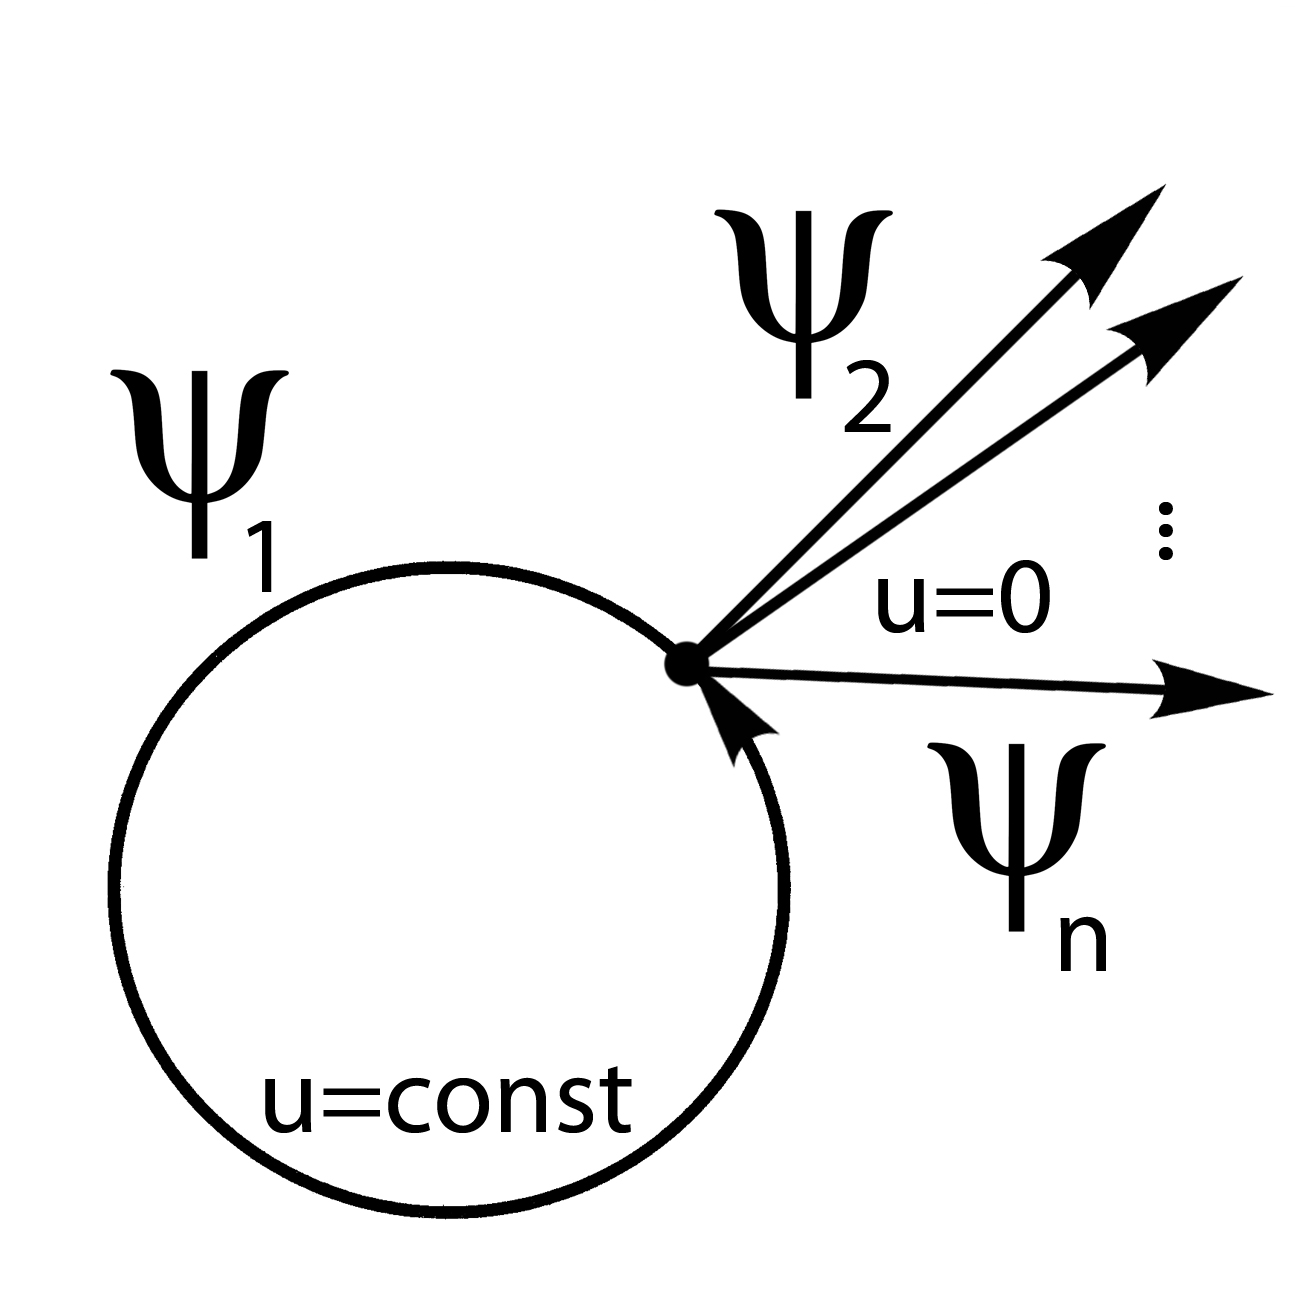
\includegraphics[scale=0.5]{n-arrow.jpg}
   \end{figure}
   \[ A = \left(\begin{smallmatrix}
   1-e^{\sqrt{u-k^2}} & 1-e^{-\sqrt{u-k^2}} & 0 & 0 & \ldots & 0 \\
   1 & 1 & -1  & 0 & \ldots & 0 \\
   1 & 1 & 0  & -1 & \ldots & 0 \\
   \vdots & \vdots & \vdots  & \vdots & \ddots & \vdots \\
   1 & 1 & 0  & 0 & \ldots & -1 \\
   \sqrt{u-k^2}-\sqrt{u-k^2} \cdot e^{\sqrt{u-k^2}} & -\sqrt{u-k^2}+\sqrt{u-k^2} \cdot e^{\sqrt{u-k^2}} & ik & \ldots & \ldots & ik
   \end{smallmatrix}\right)\]
   и набором правых частей:
   \[b = \left(\begin{smallmatrix}
   0 \\
   1 \\
   0 \\
   \vdots \\
   0 \\
   ik
   \end{smallmatrix}\right), \ 
   \left(\begin{smallmatrix}
   0 \\
   0 \\
   1 \\
   \vdots \\
   0 \\
   ik
   \end{smallmatrix}\right), \ldots
   \left(\begin{smallmatrix}
   0 \\
   0 \\
   0 \\
   \vdots \\
   1 \\
   ik
   \end{smallmatrix}\right).
   \]
   Решая первую СЛАУ относительно $C_1, C_2, C_3, C_5, \ldots, C_{2n-1}$ с различными правыми частями, будем последовательно получать строки матрицы рассеяния: 
   
   \begin{itemize}
   	\item $C_3 = R_{22}, \ C_5 = T_{23}, \ldots, C_{2n-1} = T_{2 \ 2n-1}$ 
   	\item $C_3 = T_{32}, \ C_5 = R_{33}, \ldots, C_{2n-1} = T_{3 \ 2n-1} $
   	\item $\cdots$ 
   	\item $C_3 = T_{2n-1 \ 2}, \ C_5 = T_{2n-1 \ 3}, \ldots, C_{2n-1} = R_{2n-1 \  2n-1}$ 
   \end{itemize}
    
   \pagebreak
    
   \subsection{КОЛЬЦО С $n$ ПОЛУБЕСКОНЕЧНЫМИ ДУГАМИ}
   Также определённый интерес представляет задача рассеяния на кольцах с $n$ полубесконечными дугами. В качестве примера рассмотрим следующий граф с 3 рёбрами единичной длины, на компактной части задан константный потенциал:
   \begin{figure}[h]
   	\centering
   	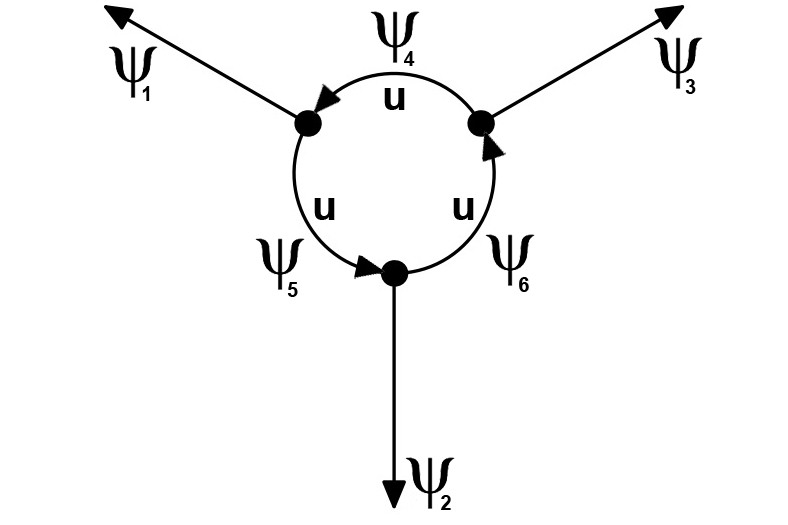
\includegraphics[scale=0.5]{arrow_graph.jpg}
   \end{figure}
   
   Ищем решение в виде
   \[\psi\left(k\right) = \left\{\psi_1\left(k,x\right), \psi_2\left(k,x\right)\right\}, \psi_3\left(k,x\right),\psi_4\left(k,x\right),\psi_5\left(k,x\right),\psi_6\left(k,x\right),\ \text{где}\]
   \[\psi_1 = c_1 \cdot e^{ikx} + c_2 \cdot e^{-ikx}, \ x \in \left[0,1\right],\]
   \[\psi_2 = c_3 \cdot e^{ikx} + c_4 \cdot e^{-ikx}, \ x \in \left[0,1\right],\]
   \[\psi_3 = c_5 \cdot e^{ikx} + c_6 \cdot e^{-ikx}, \ x \in \left[0,1\right],\]
   \[\psi_4 = c_7 \cdot e^{\sqrt{u-k^2}} + c_8 \cdot e^{-\sqrt{u-k^2}}, \ x \in \left[0, +\infty\right),\]
   \[\psi_5 = c_9 \cdot e^{\sqrt{u-k^2}} + c_{10} \cdot e^{-\sqrt{u-k^2}}, \ x \in \left[0, +\infty\right),\]
   \[\psi_6 = c_{11} \cdot e^{\sqrt{u-k^2}} + c_{12} \cdot e^{-\sqrt{u-k^2}}, \ x \in \left[0, +\infty\right).\]
   Обозначив $p = \sqrt{u-k^2}$, получим сопутствующую систему законов Кирхгофа с нулевой правой частью:
   \[ A = \left(\begin{smallmatrix}
   1 & 1 & 0 & 0 & 0 & 0 & -e^{p} & -e^{-p} & 0 & 0 & 0 & 0 \\
   1 & 1 & 0 & 0 & 0 & 0 & 0 & 0 & -1 & -1 & 0 & 0 \\
   ik & -ik & 0 & 0 & 0 & 0 & -pe^{p} & pe^{-p} & p & -p & 0 & 0\\
   0 & 0 & 1 & 1 & 0 & 0 & 0 & 0 & -e^{p} & -e^{-p} & 0 & 0 \\
   0 & 0 & 1 & 1 & 0 & 0 & 0 & 0 & 0 & 0 & -1 & -1 \\
   0 & 0 & ik & -ik & 0 & 0 & 0 & 0 & -pe^{p} & pe^{-p} & p & -p \\
   0 & 0 & 0 & 0 & 1 & 1 & 0 & 0 & 0 & 0 & -e^{p} & -e^{-p} \\
   0 & 0 & 0 & 0 & 1 & 1 & -1 & -1 & 0 & 0 & 0 & 0 \\
   0 & 0 & 0 & 0 & ik & -ik & p & -p & 0 & 0 & -pe^{p} & pe^{-p} \\
   \end{smallmatrix}\right)\]
   Подставляя поочерёдно в эту систему наборы 
   \[
   \begin{cases}
   c_1 = R_{11},\\
   c_2 = 1, \\
   c_3 = T_{12}, \\
   c_4 = 0, \\
   c_5 = T_{13}, \\
   c_6 = 0,
   \end{cases}, \ 
   \begin{cases}
   c_1 = T_{21},\\
   c_2 = 0, \\
   c_3 = R_{12}, \\
   c_4 = 1, \\
   c_5 = T_{23}, \\
   c_6 = 0,
   \end{cases}, \
   \begin{cases}
   c_1 = T_{31},\\
   c_2 = 0, \\
   c_3 = T_{32}, \\
   c_4 = 0, \\
   c_5 = R_{13}, \\
   c_6 = 1,
   \end{cases}
   \]
   получим искомые данные рассеяния:
   \begin{itemize}
  	 \item $C_1 = R_{11}, C_3 = T_{12}, C_5 = T_{13}$, 
  	 \item $C_1 = T_{21}, C_3 = R_{22}, C_5 = T_{23}$,  
 	 \item $C_1 = T_{31}, C_3 = T_{32}, C_5 = R_{33}$.
   \end{itemize}

   TODO: выписать явный вид решений
   
   \pagebreak
   
   \section{СПЕКТРАЛЬНАЯ ХИРУРГИЯ КВАНТОВЫХ ГРАФОВ}
   Основным приложением теории квантового рассеяния является моделирование полупроводниковых структур. Но в настоящих полупроводниках число молекул очень велико! Поэтому для решения задач моделирования используют методы хирургии квантовых графов. Основная идея данных методов заключается в том, что сначала решается дифференциальная задача рассеяния на примитивном графе, а затем примитивы склеиваются друг с другом согласно некоторому правилу с известным преобразованием данных рассеяния.
   
   В работе А.~Н.~Бондаренко и В.~А.~Дедка \cite{SpectralSurgery} рассмотрен метод склейки графов, содержащих неизвестную компактную часть и две бесконечные дуги. Предполагается, что потенциалы на бесконечных рёбрах нулевые.
   \begin{figure}[!htb]
   	\centering
   	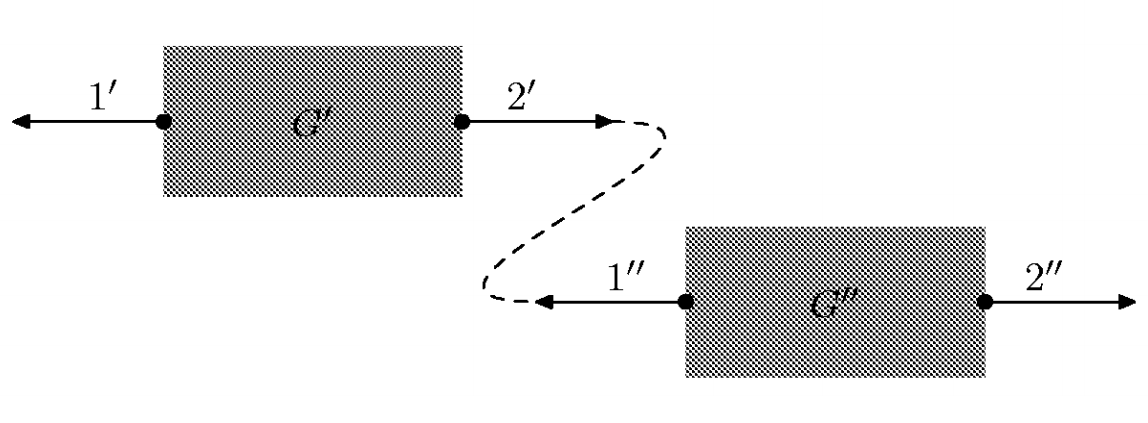
\includegraphics[scale=0.3]{skleika1.png}
   \end{figure}

   Была поставлена задача: рассмотреть процесс склейки двух графов, содержащих неизвестную компактную часть и три полубесконечных дуги, по двум парам дуг.
   
   \subsection{СКЛЕЙКА ПАРЫ ГРАФОВ С ОДИНАКОВЫМИ ДАННЫМИ РАССЕЯНИЯ}
   \begin{figure}[!htb]
   	\centering
   	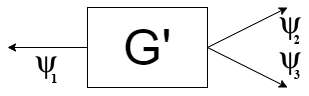
\includegraphics[scale=0.5]{g_prime.png}
   \end{figure}

   Рассмотрим граф $G^\prime$, его данные рассеяния известны. Для решения поставленной задачи построим рассеивающий оператор $SC$, сопоставляющий решениям с двух правых бесконечных дуг решение на левой бесконечной дуге.
   
   Поскольку мы знаем общий вид решения на полубесконечных дугах
   \begin{equation}
   \begin{split}
   \label{GeneralSolution1}
   \psi_1\left(x\right) &= a e^{-ikx} + b e^{ikx}, \\
   \psi_2\left(x\right) &= c e^{-ikx} + d e^{ikx}, \\
   \psi_3\left(x\right) &= e e^{-ikx} + f e^{ikx},
   \end{split}
   \end{equation}

   то наша задача состоит в построении линейного оператора $SC$, такого что:
   \[SC\left(
   \begin{array}{c}
   c \\
   d \\
   e \\
   f
   \end{array}\right) = \left(\begin{array}{c}
   a \\
   b
   \end{array}\right)\]
   
   Разложим волновые функции по всевозможным исходам:
   \begin{equation}
   \label{GeneralSolution2}
   \begin{aligned}
   \psi_1(x) &= \alpha\left(e^{-ikx} + Re^{ikx}\right) + \beta\left(Te^{ikx}\right) + \gamma \left(Te^{ikx}\right) = \\
   &= \alpha e^{-ikx} + \left(\alpha R + \beta T + \gamma T\right) e^{ikx}, \\
   \psi_2(x) &= \alpha \left(T e^{ikx}\right) + \beta \left(e^{-ikx} + R e^{ikx}\right) + \gamma \left(T e^{ikx}\right) = \\
   &= \beta e^{-ikx} + \left(\alpha T + \beta R + \gamma T\right) e^{ikx}, \\
   \psi_3(x) &= \alpha \left(T e^{ikx}\right) + \beta \left(T e^{ikx}\right) + \gamma \left(e^{-ikx} + R e^{ikx}\right) = \\
   &= \gamma e^{-ikx} + \left(\alpha T + \beta T + \gamma R\right) e^{ikx}.
   \end{aligned}
   \end{equation}
   
   Тогда из (\ref{GeneralSolution1}) и (\ref{GeneralSolution2}) получим СЛАУ на $a, b, c, d, e, f$:

   \[
   \begin{cases}
   a = \alpha, \\
   b = \alpha R + \beta T + \gamma T, \\
   c = \beta, \\
   d = \alpha T + \beta R + \gamma T, \\
   e = \gamma, \\
   f = \alpha T + \beta T + \gamma R.
   \end{cases}
   \]
   Выражая $a, b$ через $c, d, e, f$, получим:
   \[
   \begin{aligned}
   a &= \left(f - cT - eR\right)T^{-1} \\
   b &= \left(f - cT - eR\right)T^{-1}R + cT + eT
   \end{aligned}
   \]
   А также условие совместности:
   \begin{equation}
   \label{compabilityCondition}
   f - cT - eR = d - cR - eT
   \end{equation}
   
   Тогда
   \[
   \begin{aligned}
   SC\left(
   \begin{array}{c}
   c \\
   d \\
   e \\
   f
   \end{array}\right) &= \left(\begin{array}{c}
   a \\
   b
   \end{array}\right) = 
   \left(\begin{array}{c}
   \left(f - cT - eR\right)T^{-1} \\
   \left(f - cT - eR\right)T^{-1}R + cT + eT
   \end{array}\right) =\\
   &= \left(\begin{array}{cccc}
   -1 & 0 & -RT^{-1} & T^{-1} \\
   T-R & 0 & T-RT^{-1}R & T^{-1}R
   \end{array}\right)
   \left(\begin{array}{c}
   c \\
   d \\
   e \\
   f
   \end{array}\right)
   \end{aligned}\]
   
   Приступим к слейке графов $G^\prime$ и $G^{\prime \prime}$:
   \begin{figure}[!htb]
   	\centering
   	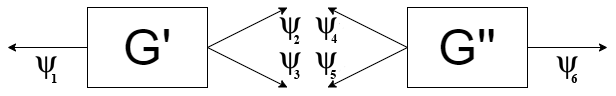
\includegraphics[scale=0.54]{skleika2.png} \\
   	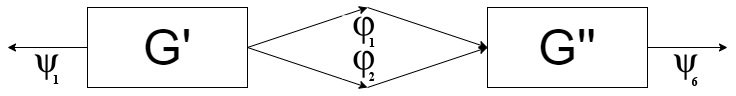
\includegraphics[scale=0.45]{skleika3.png}
   \end{figure}

   Ясно, что $\psi_1\left(x\right), \varphi_1\left(x\right), \varphi_1\left(1-x\right), \varphi_2\left(x\right), \varphi_2\left(1-x\right), \psi_2\left(x\right)$ ~--- решения задач рассеяния для графов  $G^\prime$ и $G^{\prime \prime}$ на полубесконечных дугах.
   
   Пусть решения на склеенном графе определены следующим образом:
   \begin{itemize}
   	\item $ \psi_1\left(x\right) = e^{-ikx} + R^\prime e^{ikx} $
   	\item $ \varphi_1\left(x\right)  = a e^{-ikx} + b e^{ikx} $
   	\item $ \varphi_2\left(x\right) = c e^{-ikx} + d e^{ikx} $
   	\item $ \psi_2\left(x\right) = T^\prime e^{ikx}$
   \end{itemize}
   Заметим, что
   \[
   \begin{aligned}
   \varphi_1\left(1-x\right) &= b e^{ik} e^{-ikx} + a e^{-ik} e^{ikx}, \\
   \varphi_2\left(1-x\right) &= d e^{ik} e^{-ikx} + c e^{-ik} e^{ikx},
   \end{aligned}\]
   
   Тогда
   \begin{equation}
   \label{boundaryCond1}
   SC\left(
   \begin{array}{c}
   a \\
   b \\
   c \\
   d
   \end{array}\right) = \left(\begin{array}{c}
   1 \\
   R^\prime
   \end{array}\right),
   \end{equation}
   \begin{equation}
   \label{boundaryCond2}
   SC\left(
   \begin{array}{c}
   b e^{ik} \\
   a e^{-ik}\\
   d e^{ik}\\
   c e^{-ik}
   \end{array}\right) = \left(\begin{array}{c}
   0 \\
   T^\prime
   \end{array}\right)   
   \end{equation}
   Отсюда получаем два уравнения на коэффициенты $a, b, c, d$:
   \[
   \begin{aligned}
   \left(d - aT -cR\right)T^{-1} &= 1 \\
   \left(c e^{-ik} - b e^{ik} T - d e^{ik}R\right) T^{-1} &= 0
   \end{aligned}\]
   
   Оставшиеся 2 уравнения получим из условия совместности (\ref{compabilityCondition}) для оператора $SC$:
   \[
   \begin{aligned}
   d - aT -cR &= b - aR - cT \\
   c e^{-ik} - b e^{ik}T - d e^{ik} R &= a e^{-ik} - b e^{ik}R - d e^{ik} T
   \end{aligned}
   \]
   Запишем получившуюся СЛАУ в матричном виде:
   \[
   \begin{pmatrix}
   -T & 0 & -R & 1\\ 
   0 & -e^{ik}T  & e^{-ik} &-e^{ik}R \\ 
   R-T & -1 & T-R & 1\\ 
   -e^{-ik} & e^{ik}\left(R-T\right) & e^{-ik} & e^{ik}\left(T-R\right)
   \end{pmatrix}
   \begin{pmatrix}
   a \\
   b \\
   c \\
   d
   \end{pmatrix} = 
   \begin{pmatrix}
   T \\
   0 \\
   0 \\
   0 
   \end{pmatrix}\]
   
   Зная решение этой системы,\[
   \left(\begin{array}{c}
   a \\
   b \\
   c \\
   d
   \end{array} \right) = 
   \left( \begin {array}{c} -{\frac { \left( R+T \right) {{\rm e}^{ik}}T
   	}{-{{\rm e}^{-ik}}+ \left(R+T\right)^2 {{\rm e}^{ik}
   }}}\\ \noalign{\medskip}-{\frac {{{\rm e}^{-ik}}T}{-{{\rm e}^{-ik}}+
   		\left(R+T\right)^2 {{\rm e}^{ik}}}}
   \\ \noalign{\medskip}-{\frac { \left( R+T \right) {{\rm e}^{ik}}T}{-{
   			{\rm e}^{-ik}}+ \left(R+T\right)^2 {{\rm e}^{ik}}}}
   \\ \noalign{\medskip}-{\frac {{{\rm e}^{-ik}}T}{-{{\rm e}^{-ik}}+
   		\left(R+T\right)^2 {{\rm e}^{ik}}}}\end {array}
   \right) 
   \]
   Из соотношения (\ref{boundaryCond1}) получим искомое значение коэффициента $R^\prime$:

   \[
   R^\prime = {\frac {-{{\rm e}^{-ik}}R+{{\rm e}^{ik}} \left( R-T \right)  \left( R+
   		2\,T \right)  \left( R+T \right) }{-{{\rm e}^{-ik}}+ \left( R+T\right)^2 {{\rm e}^{ik}}}}
   \]
   Аналогично, из соотношения (\ref{boundaryCond2}) получим $T^\prime$:
   \[
   T^\prime = {\frac {-2{T}^{2}}{-{{\rm e}^{-ik}}+ \left(R+T\right)^2 {{\rm e}^{ik}}}}
   \]
   
   Однако приведённые выше выкладки верны только при выполнении условий $T \neq 0$ и $-e^{-ik} + \left(R+T\right)^2 e^{ik} \neq 0$. Рассмотрим их подробнее.
   
   Условие $T = 0$ эквивалентно полному отражению волны при попадании частицы в компактную часть графа при движениии по полубесконечному ребру. Поскольку склеиваемые графы $G^\prime$ и $G^{\prime\prime}$ имеют одинаковые данные рассеяния, то итоговая $S$-матрица будет иметь вид:
   \[
   S(k)=\left(%
   \begin{array}{cc}
   -1 & 0 \\
   0 & -1 \\
   \end{array}%
   \right)
   \]
   
   Условие $-e^{-ik} + \left(R+T\right)^2 e^{ik} \neq 0$ может показаться недостижимым при добавлении условия нормировки $RR^* +TT^* +TT^* = 1$, однако можно подобрать такие значения $R, \ T, \ k$, что знаменатель обратится в нуль, но при этом будет выполнено условие нормировки. Чтобы показать это, перепишем неравенство:
   \[
   \begin{aligned}
   -e^{-ik} + \left(R+T\right)^2 e^{ik} &\neq 0 \\
   \left(R+T\right)^2 e^{ik} &= e^{-ik} \\
   \left(R+T\right)^2 &= e^{-2ik} \\
   R+T &= e^{-ik} \\
   T &= -R + e^{-ik}
   \end{aligned}
   \]
   
   И подставим полученное выражение для $T$ в условие нормировки:
   
   \[
   \begin{aligned}
   RR^* + 2TT^* &= 1\\
   RR^* + 2\left(-R + e^{-ik}\right)\left(-R^* + e^{ik}\right) &= 1
   \end{aligned}\]
   \[
   \begin{aligned}
   RR^* + 2\left(RR^* -Re^{ik} -R^*e^{-ik} + 1\right) &= 1\\
   3RR^* -2Re^{ik}-2R^*e^{-ik} &= -1
   \end{aligned}
   \]
   
   Запишем коэффициент отражения в показательной форме: $R = \rho e^{i \varphi}$.
   
   Тогда полученное ранее выражение примет вид:
   \[
   3 \rho^2 -2 \rho e^{i\left(\varphi+k\right)} -2 \rho e^{-i\left(\varphi+k\right)} = 1
   \]
   
   Выберем $\varphi$ таким образом, чтобы $\varphi + k = 0$. Тогда определим $\rho$ из квадратного уравнения $3\rho^2 -4\rho -1 = 0$.
   Это уравнение имеет один положительный корень. Значит, удалось подобрать такие $R, \ T, \ k$, при которых полученное правило склейки не работает. Возможно, условие $-e^{-ik} + \left(R+T\right)^2 e^{ik} \neq 0$ всё же будет являться недостижимым в задачах рассеяния, но для того, чтобы показать это, нужно привлекать дополнительные соображения.
   
   Таким образом, доказана
   
   \begin{theorem}
   	Пусть даны два одинаковых графа $G^\prime, \ G^{\prime\prime}$, содержащих три полубесконечных дуги и неизвестную компактную часть. Пусть для данных рассеяния графов  $G^\prime, \ G^{\prime\prime}$ выполнено условие совместности. Пусть также $T \neq 0, \ R+T \neq e^{-ik}$
   	
   	Тогда данные рассеяния графа, полученного склейкой графов $G^\prime, \ G^{\prime\prime}$ по двум полубесконечным дугам в дугу единичной длины, имеют вид $\left(\begin{matrix}
   	R^\prime & T^\prime \\
   	T^\prime & R^\prime
   	\end{matrix}\right)$, где
   	\[
   	\begin{aligned}
   	R^\prime &= {\frac {-{{\rm e}^{-ik}}R+{{\rm e}^{ik}} \left( R-T \right)  \left( R+
		2\,T \right)  \left( R+T \right) }{-{{\rm e}^{-ik}}+ \left(R+T\right)^2 {{\rm e}^{ik}}}}, \\
    T^\prime &= {\frac {-2{T}^{2}}{-{{\rm e}^{-ik}}+ \left(R+T\right)^2 {{\rm e}^{ik}}}}.
   	\end{aligned}\]
   \end{theorem}

   \subsection{СКЛЕЙКА ПАРЫ ГРАФОВ С ПРОИЗВОЛЬНЫМИ ДАННЫМИ РАССЕЯНИЯ}
   
   Обобщим полученный результат на случай пары графов, содержащих 3 полубесконечных дуги, имеющих произвольные данные рассеяния.
   
   \begin{figure}[!htb]
   	\centering
   	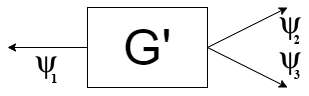
\includegraphics[scale=0.5]{g_prime.png}
   \end{figure}
   
   Аналогично предыдущему пункту, рассмотрим граф $G^\prime$ с известными данными рассеяния 
   \[
      S^\prime(k)=\left(%
   \begin{array}{cc}
   R_{11}^\prime & T_{12}^\prime \\
   T_{21}^\prime & R_{22}^\prime \\
   \end{array}%
   \right).
   \]
   
   Построим рассеивающий оператор $SC_{rl}^\prime$, \ сопоставляющий решениям с двух правых полубесконечных дуг решение на левой полубесконечной дуге.
   
   Общий вид решений на полубесконечных дугах известен:
   \begin{equation}
   \label{GeneralizedSolution1}
   \begin{split}
   \psi_1\left(x\right) &= a e^{-ikx} + b e^{ikx}, \\
   \psi_2\left(x\right) &= c e^{-ikx} + d e^{ikx}, \\
   \psi_3\left(x\right) &= e e^{-ikx} + f e^{ikx},
   \end{split}
   \end{equation}
   
   Будем строить линейный оператор $SC_{rl}^\prime$, \ удовлетворяющий условию:
   \[SC_{rl}^\prime\left(
   \begin{array}{c}
   c \\
   d \\
   e \\
   f
   \end{array}\right) = \left(\begin{array}{c}
   a \\
   b
   \end{array}\right)\]
   
   Раскладывая волновые функции по всевозможным исходам,
   \begin{equation}
   \label{GeneralizedSolution2}
   \begin{aligned}
   \psi_1(x) &= \alpha\left(e^{-ikx} + R_{11}^\prime e^{ikx}\right) + \beta\left(T_{21}^\prime e^{ikx}\right) + \gamma \left(T_{31}^\prime e^{ikx}\right) = \\
   &= \alpha e^{-ikx} + \left(\alpha R_{11}^\prime  + \beta T_{21}^\prime  + \gamma T_{31}^\prime \right) e^{ikx}, \\
   \psi_2(x) &= \alpha \left(T_{12}^\prime  e^{ikx}\right) + \beta \left(e^{-ikx} + R_{22}^\prime  e^{ikx}\right) + \gamma \left(T_{32}^\prime  e^{ikx}\right) = \\
   &= \beta e^{-ikx} + \left(\alpha T_{12}^\prime  + \beta R_{22}^\prime  + \gamma T_{32}^\prime \right) e^{ikx}, \\
   \psi_3(x) &= \alpha \left(T_{13}^\prime  e^{ikx}\right) + \beta \left(T_{23}^\prime  e^{ikx}\right) + \gamma \left(e^{-ikx} + R_{33}^\prime  e^{ikx}\right) = \\
   &= \gamma e^{-ikx} + \left(\alpha T_{13}^\prime  + \beta T_{23}^\prime  + \gamma R_{33}^\prime \right) e^{ikx}.
   \end{aligned}
   \end{equation}
   
   Из (\ref{GeneralizedSolution1}) и (\ref{GeneralizedSolution2}) получим СЛАУ на $a, b, c, d, e, f$:
   
   \[
   \begin{cases}
   a = \alpha, \\
   b = \alpha R_{11}^\prime  + \beta T_{21}^\prime  + \gamma T_{31}^\prime , \\
   c = \beta, \\
   d = \alpha T_{12}^\prime  + \beta R_{22}^\prime  + \gamma T_{32}^\prime , \\
   e = \gamma, \\
   f = \alpha T_{13}^\prime  + \beta T_{23}^\prime  + \gamma R_{33}.
   \end{cases}
   \]
   
   Выражая $a, b$ через $c, d, e, f$, получим:
   \[
   \begin{aligned}
   a &= \left(f - cT_{23}^\prime  - eR_{33}^\prime \right)\left(T_{13}^\prime\right)^{-1} \\
   b &= \left(f - cT_{23}^\prime  - eR_{33}^\prime \right)\left(T_{13}^\prime\right)^{-1}R_{11}^\prime + cT_{21}^\prime + eT_{31}^\prime
   \end{aligned}
   \]
   С необходимым условием совместности:
   \begin{equation}
   \label{compabilityConditionGeneralized}
   \left(f - cT_{23}^\prime - eR_{33}^\prime\right)\left(T_{13}^\prime\right)^{-1} = \left(d - cR_{22}^\prime - eT_{32}^\prime\right)\left(T_{12}^\prime\right)^{-1}.
   \end{equation}
   
   Тогда
   \[
   \begin{aligned}
   SC_{rl}^\prime\left(
   \begin{array}{c}
   c \\
   d \\
   e \\
   f
   \end{array}\right) &= \left(\begin{array}{c}
   a \\
   b
   \end{array}\right) = 
   \left(\begin{array}{c}
   \left(f - cT_{23}^\prime - eR_{33}^\prime\right)\left(T_{13}^\prime\right)^{-1} \\
   \left(f - cT_{23}^\prime - eR_{33}^\prime\right)\left(T_{13}^\prime\right)^{-1}R_{11}^\prime + cT_{21}^\prime + eT_{31}^\prime
   \end{array}\right) =\\
   &= \left(\begin{array}{cccc}
   -T_{23}^\prime T_{13}^\prime & 0 & -R_{33}^\prime \left(T_{13}^\prime\right)^{-1} & \left(T_{13}^\prime\right)^{-1} \\
   T_{21}^\prime- T_{23}^\prime\left(T_{13}^\prime\right)^{-1}R_{11}^\prime & 0 & T_{31}^\prime - R_{33}^\prime \left(T_{13}^\prime\right)^{-1}R_{11}^\prime & \left(T_{13}^\prime\right)^{-1}R_{11}^\prime
   \end{array}\right)
   \left(\begin{array}{c}
   c \\
   d \\
   e \\
   f
   \end{array}\right)
   \end{aligned}\]
   
   Далее будет производиться склейка графа $G^\prime$ с графом $G^{\prime\prime}$, имеющим три полубесконечных дуги, неизвестную компактную часть, а также известные данные рассеяния 
   \[
   S^{\prime\prime}(k)=\left(%
   \begin{array}{cc}
   R_{11}^{\prime\prime} & T_{12}^{\prime\prime} \\
   T_{21}^{\prime\prime} & R_{22}^{\prime\prime} \\
   \end{array}%
   \right).
   \]
   
   Для этого понадобится оператор $SC_{lr}^{\prime\prime}$, \ сопоставляющий решениям с двух левых полубесконечных дуг графа $G^{\prime\prime}$ решение на правой полубесконечной дуге. Очевидно, что
    \[
   \begin{aligned}
   SC_{rl}^{\prime\prime}\left(
   \begin{array}{c}
   c \\
   d \\
   e \\
   f
   \end{array}\right) &= \left(\begin{array}{cccc}
   -T_{23}^{\prime\prime} T_{13}^{\prime\prime} & 0 & -R_{33}^{\prime\prime} \left(T_{13}^{\prime\prime}\right)^{-1} & \left(T_{13}^{\prime\prime}\right)^{-1} \\
   T_{21}^{\prime\prime}- T_{23}^{\prime\prime}\left(T_{13}^{\prime\prime}\right)^{-1}R_{11}^{\prime\prime} & 0 & T_{31}^{\prime\prime} - R_{33}^{\prime\prime} \left(T_{13}^{\prime\prime}\right)^{-1}R_{11}^{\prime\prime} & \left(T_{13}^{\prime\prime}\right)^{-1}R_{11}^{\prime\prime}
   \end{array}\right)
   \left(\begin{array}{c}
   c \\
   d \\
   e \\
   f
   \end{array}\right).
   \end{aligned}\]
   
   Приступим к слейке графов $G^\prime$ и $G^{\prime \prime}$:
   \begin{figure}[!htb]
   	\centering
   	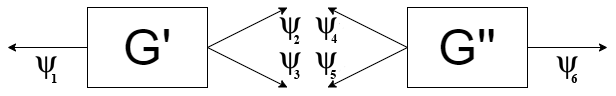
\includegraphics[scale=0.54]{skleika2.png} \\
   	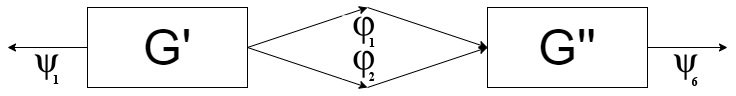
\includegraphics[scale=0.45]{skleika3.png}
   \end{figure}
   
   Ясно, что $\psi_1\left(x\right), \varphi_1\left(x\right), \varphi_1\left(1-x\right), \varphi_2\left(x\right), \varphi_2\left(1-x\right), \psi_2\left(x\right)$ ~--- решения задач рассеяния для графов  $G^\prime$ и $G^{\prime \prime}$ на полубесконечных дугах.
   
   Пусть решения на склеенном графе определены следующим образом:
   \begin{itemize}
   	\item $ \psi_1\left(x\right) = e^{-ikx} + R_{11} e^{ikx} $
   	\item $ \varphi_1\left(x\right)  = a e^{-ikx} + b e^{ikx} $
   	\item $ \varphi_2\left(x\right) = c e^{-ikx} + d e^{ikx} $
   	\item $ \psi_2\left(x\right) = T_{12} e^{ikx}$
   \end{itemize}
    Заметим, что
   \[
   \begin{aligned}
   \varphi_1\left(l_1-x\right) &= b e^{ikl_1} e^{-ikx} + a e^{-ikl_1} e^{ikx}, \\
   \varphi_2\left(l_2-x\right) &= d e^{ikl_2} e^{-ikx} + c e^{-ikl_2} e^{ikx},
   \end{aligned}\]
   
   Тогда
   \begin{equation}
   \label{generalizedBoundaryCond1}
   SC_{rl}^\prime\left(
   \begin{array}{c}
   a \\
   b \\
   c \\
   d
   \end{array}\right) = \left(\begin{array}{c}
   1 \\
   R_{11}
   \end{array}\right),
   \end{equation}
   
   \begin{equation}
   \label{generalizedBoundaryCond2}
   SC_{lr}^{\prime\prime}\left(
   \begin{array}{c}
   b e^{ikl_1} \\
   a e^{-ikl_1}\\
   d e^{ikl_2}\\
   c e^{-ikl_2}
   \end{array}\right) = \left(\begin{array}{c}
   0 \\
   T_{12}
   \end{array}\right)   
   \end{equation}
   
   Отсюда получаем два уравнения на коэффициенты $a, b, c, d$:
   \[
   \begin{aligned}
   -T_{23}^\prime T_{13}^\prime a - R_{33}^\prime \left(T_{13}^\prime\right)^{-1}c + \left(T_{13}^\prime\right)^{-1}d &= 1 \\
   -T_{23}^{\prime\prime} T_{13}^{\prime\prime} b e^{ikl_1} - R_{33}^{\prime\prime} \left(T_{13}^{\prime\prime}\right)^{-1}d e^{ikl_2} + \left(T_{13}^{\prime\prime}\right)^{-1}c e^{-ikl_2} &= 0
   \end{aligned}\]
   
   Оставшиеся 2 уравнения получим из условия совместности (\ref{compabilityConditionGeneralized}) для операторов $SC_{rl}^\prime, \ SC_{lr}^{\prime\prime}$:
   \[
   \begin{aligned}
   \left(d-aT_{23}^\prime -cR_{33}^\prime\right)\left(T_{13}^\prime\right)^{-1} &= \left(b-aR_{22}^\prime -c T_{32}^\prime\right)\left(T_{12}^\prime\right)^{-1} \\
   \left(c e^{-ikl_2}-b e^{ikl_1} T_{23}^{\prime\prime}-d e^{ikl_2}R_{33}^{\prime\prime}\right)\left(T_{13}\right)^{-1} &= \left(a e^{-ikl_1} - b e^{ikl_1} R_{22}^{\prime\prime} -d e^{ikl_2} T_{32}^{\prime\prime}\right)\left(T_{12}^{\prime\prime}\right)^{-1}
   \end{aligned}
   \]
   
   Перепишем СЛАУ в матричном виде:
   \[
   \begin{pmatrix}
   -T_{23}^{\prime}T_{13}^{\prime} & 0 & -\frac{R_{33}^{\prime}}{T_{13}^\prime} & \frac{1}{T_{13}^\prime}\\ 
   0 & -T_{23}^{\prime\prime} T_{13}^{\prime\prime} e^{ikl_1}  & \frac{e^{-ikl_2}}{T_{13}^{\prime\prime}} & -\frac{R_{33}^{\prime\prime}e^{ikl_2}}{T_{13}^{\prime\prime}} \\ 
   \frac{R_{22}^{\prime}}{T_{12}^{\prime}}-\frac{T_{23}^{\prime}}{T_{13}^{\prime}} & -\frac{1}{T_{12}^{\prime}} & \frac{T_{32}^{\prime}}{T_{12}^{\prime}}-\frac{R_{33}^{\prime}}{T_{13}^{\prime}} & \frac{1}{T_{13}^{\prime}}\\ 
   -\frac{e^{-ikl_1}}{T_{12}^{\prime\prime}} & e^{ikl_1}\left(\frac{R_{22}^{\prime\prime}}{T_{12}^{\prime\prime}} - \frac{T_{23}^{\prime\prime}}{T_{13}^{\prime\prime}}\right) & e^{-ikl_2} & e^{ikl_2}\left(\frac{T_{32}^{\prime\prime}}{T_{12}^{\prime\prime}} - \frac{R_{33}^{\prime\prime}}{T_{13}^{\prime\prime}}\right)
   \end{pmatrix}
   \begin{pmatrix}
   a \\
   b \\
   c \\
   d
   \end{pmatrix} = 
   \begin{pmatrix}
   1 \\
   0 \\
   0 \\
   0 
   \end{pmatrix}\]
   
   Решая эту систему, найдём искомое значение $R_{11}$ по формуле (\ref{generalizedBoundaryCond1}):   	
   {\tiny
   \[
   {\frac {{\it T_{13}^{\prime}}\, \left( -{\it R_{33}^{\prime\prime}}\,{\it T_{13}^{\prime\prime}}\, \left( {\it R_{11}^{\prime}}\,{
   			\it R_{33}^{\prime}}-{\it T_{13}^{\prime}}\,{\it T_{31}^{\prime}} \right) {{\rm e}^{-ik \left( {\it l1}-{
   					\it l2} \right) }}- \left( {\it T_{12}^{\prime\prime}}\,{{\it T_{13}^{\prime\prime}}}^{3}{\it T_{23}^{\prime\prime}}+{\it 
   			R_{22}^{\prime\prime}}\,{\it T_{13}^{\prime\prime}}-{\it T_{12}^{\prime\prime}}\,{\it T_{23}^{\prime\prime}} \right)  \left( {\it R_{11}^{\prime}}\,{\it 
   			R_{22}^{\prime}}-{\it T_{12}^{\prime}}\,{\it T_{21}^{\prime}} \right) {{\rm e}^{ik \left( {\it l1}-{\it l2
   				} \right) }}+{{\rm e}^{-ik \left( {\it l1}+{\it l2} \right) }}{\it T_{13}^{\prime\prime}
   		}\,{\it R_{11}^{\prime}}+ \left(  \left( -{\it R_{22}^{\prime}}\,{\it T_{31}^{\prime}}+{\it T_{21}^{\prime}}\,{\it T_{32}^{\prime}
   		} \right) {\it T_{13}^{\prime}}+ \left( -{\it R_{11}^{\prime}}\,{\it T_{32}^{\prime}}+{\it T_{12}^{\prime}}\,{\it T_{31}^{\prime}}
   		\right) {\it T_{23}^{\prime}}+{\it R_{33}^{\prime}}\, \left( {\it R_{11}^{\prime}}\,{\it R_{22}^{\prime}}-{\it T_{12}^{\prime}}\,
   		{\it T_{21}^{\prime}} \right)  \right)  \left( {\it R_{33}^{\prime\prime}}\,{\it T_{12}^{\prime\prime}}\,{{\it T_{13}^{\prime\prime}}}^{
   			2}{\it T_{23}^{\prime\prime}}-{{\it T_{13}^{\prime\prime}}}^{3}{\it T_{23}^{\prime\prime}}\,{\it T_{32}^{\prime\prime}}+{\it R_{22}^{\prime\prime}}\,{\it R_{33}^{\prime\prime}}\,
   		{\it T_{13}^{\prime\prime}}-{\it R_{33}^{\prime\prime}}\,{\it T_{12}^{\prime\prime}}\,{\it T_{23}^{\prime\prime}} \right) {{\rm e}^{ik \left( 
   				{\it l1}+{\it l2} \right) }}-{\it T_{23}^{\prime\prime}}\, \left( {\it R_{11}^{\prime}}\,{\it T_{32}^{\prime}}-{
   			\it T_{12}^{\prime}}\,{\it T_{31}^{\prime}} \right) {{\it T_{13}^{\prime\prime}}}^{3}- \left( {\it R_{33}^{\prime\prime}}\,{\it 
   			T_{12}^{\prime\prime}}+{\it T_{32}^{\prime\prime}} \right)  \left( {\it R_{11}^{\prime}}\,{\it T_{23}^{\prime}}-{\it T_{13}^{\prime}}\,{\it 
   			T_{21}^{\prime}} \right) {\it T_{13}^{\prime\prime}}+{\it R_{33}^{\prime\prime}}\,{\it T_{12}^{\prime\prime}}\, \left( {\it R_{11}^{\prime}}\,{\it 
   			T_{23}^{\prime}}-{\it T_{13}^{\prime}}\,{\it T_{21}^{\prime}} \right)  \right) }{-{{\rm e}^{-ik \left( {
   					\it l1}-{\it l2} \right) }}{\it R_{33}^{\prime\prime}}\,{\it T_{13}^{\prime\prime}}\,{\it R_{33}^{\prime}}\,{\it T_{13}^{\prime}}-
   		\left( {\it T_{12}^{\prime\prime}}\,{{\it T_{13}^{\prime\prime}}}^{3}{\it T_{23}^{\prime\prime}}+{\it R_{22}^{\prime\prime}}\,{\it T_{13}^{\prime\prime}}-{\it 
   			T_{12}^{\prime\prime}}\,{\it T_{23}^{\prime\prime}} \right)  \left( {\it T_{12}^{\prime}}\,{{\it T_{13}^{\prime}}}^{2}{\it T_{23}^{\prime}}+{
   			\it R_{22}^{\prime}}\,{\it T_{13}^{\prime}}-{\it T_{12}^{\prime}}\,{\it T_{23}^{\prime}} \right) {{\rm e}^{ik \left( {
   					\it l1}-{\it l2} \right) }}+{{\rm e}^{-ik \left( {\it l1}+{\it l2}
   				\right) }}{\it T_{13}^{\prime\prime}}\,{\it T_{13}^{\prime}}+ \left( {\it R_{33}^{\prime\prime}}\,{\it T_{12}^{\prime\prime}}\,{{\it 
   				T_{13}^{\prime\prime}}}^{2}{\it T_{23}^{\prime\prime}}-{{\it T_{13}^{\prime\prime}}}^{3}{\it T_{23}^{\prime\prime}}\,{\it T_{32}^{\prime\prime}}+{\it R_{22}^{\prime\prime}}\,{
   			\it R_{33}^{\prime\prime}}\,{\it T_{13}^{\prime\prime}}-{\it R_{33}^{\prime\prime}}\,{\it T_{12}^{\prime\prime}}\,{\it T_{23}^{\prime\prime}} \right)  \left( {
   			\it R_{33}^{\prime}}\,{\it T_{12}^{\prime}}\,{{\it T_{13}^{\prime}}}^{2}{\it T_{23}^{\prime}}-{{\it T_{13}^{\prime}}}^{3}{\it T_{23}^{\prime}}
   		\,{\it T_{32}^{\prime}}+{\it R_{22}^{\prime}}\,{\it R_{33}^{\prime}}\,{\it T_{13}^{\prime}}-{\it R_{33}^{\prime}}\,{\it T_{12}^{\prime}}\,{
   			\it T_{23}^{\prime}} \right) {{\rm e}^{ik \left( {\it l1}+{\it l2} \right) }}-{
   			\it T_{13}^{\prime}}\, \left( {\it T_{32}^{\prime}}\,{\it T_{23}^{\prime\prime}}\,{{\it T_{13}^{\prime\prime}}}^{3}+{{\it T_{13}^{\prime}}}^{2
   		}{\it T_{23}^{\prime}}\, \left( {\it R_{33}^{\prime\prime}}\,{\it T_{12}^{\prime\prime}}+{\it T_{32}^{\prime\prime}} \right) {\it T_{13}^{\prime\prime}}-{
   			{\it T_{13}^{\prime}}}^{2}{\it T_{23}^{\prime}}\,{\it R_{33}^{\prime\prime}}\,{\it T_{12}^{\prime\prime}} \right) }}
   \]
}
   

   Заметим, что подобный подход позволяет склеивать одинаковые с топологической точки зрения графы, в том числе имеющие различные данные рассеяния. Повторив вышеописанные рассуждения, можно получить теорему на данный случай.
   
   Основное преимущество данного подхода заключается в том, что для решения задачи рассеяния на полупроводниковых структурах сначала решается относительно простая дифференциальная задача для примитивного графа, а затем при помощи алгебраических операций это решение масштабируется до всего искомого графа.
   
   \section{СХОДИМОСТЬ ДАННЫХ РАССЕЯНИЯ В ПРЯМОЙ ЗАДАЧЕ РАССЕЯНИЯ}
   
   Эффективная передача света, электрического заряда, сигнала, спина, тепла в сетях требует знания об изменении волновой динамики при регулировании параметров системы. Это может быть достигнуто с помощью математических моделей, которые обеспечивают реалистичное описание переноса частиц и волн в волноводах \cite{TransparentQuantumGraphs}.
   
   Важную роль при рассеянии частицы на графе играют граничные условия и рассеивающие потенциалы. Проходя через вершину, частица формирует набор волн, распространяющихся по всем инцидентным данной вершине дугам. Накапливаясь, волны могут интерферировать друг с другом, вызывая повышенную сопротивляемость или отсутствие сопротивления при передаче сигнала.
   Например, безотражательная передача волн является одной из основных задач в теории оптоволоконных сетей.
   
   Для решения подобных задач важно понимать, как изменяются данные рассеяния при вариации потенциалов.
   
   \begin{Def}
   	Прямая задача рассеяния ~--- это вычисление $S$-матрицы по заданному  графу и набору потенциалов.
   \end{Def}

   \begin{Def}
   	Обратная задача рассеяния ~--- это вычисление набора рассеивающих потенциалов по заданному графу и $S$-матрице.
   \end{Def}

   Пусть требуется определить данные рассеяния для заданного графа и заданного измеримого потенциала. Известно, что любая измеримая функция может быть представлена в виде предела равномерно сходящейся последовательности ступенчатых функций \cite{Kolmogorov}. Поэтому важно рассматривать задачи рассеяния для ступенчатых функций.
   
   Имеет место следующая теорема:
   \begin{theorem}
   	Задача рассеяния со ступенчатым рассеивающим потенциалом эквивалентна задаче рассеяния с константными потенциалами, но с большим числом вершин.
   \end{theorem}
   \begin{proof}
   	\begin{figure}[!htb]
   		\centering
   		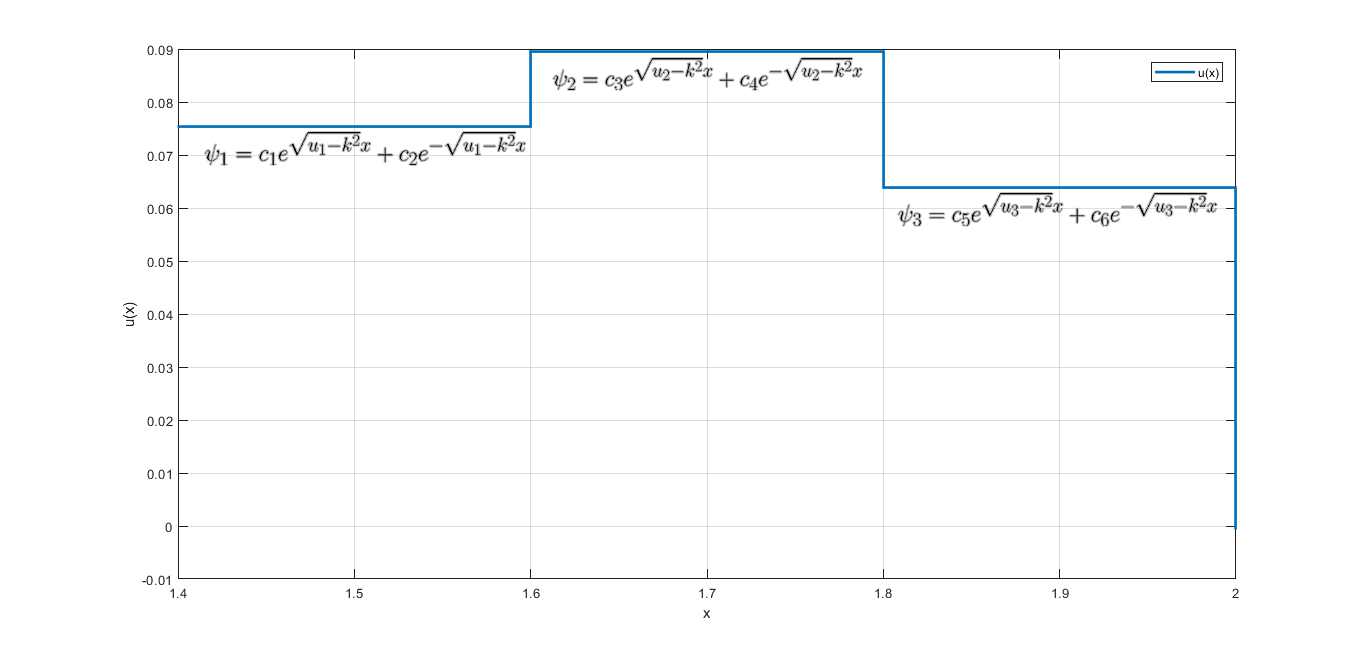
\includegraphics[scale=0.5]{step.png}
   	\end{figure}
   	Стандартным подходом к решению одномерного стационарного уравнения Шрёдингера является предположение об общем виде решений с добавлением условий стыковки: требуется непрерывность волновой функции и её производной \cite{Peisakhovich}. На каждой дуге направление задано однозначно, оно не может поменяться на каком-то подынтервале. Поэтому можно добавить фиктивные вершины в точки скачков ступенчатого потенциала, после чего получаем новую задачу рассеяния для графа с большим числом вершин, константными потенциалами. 
   \end{proof}
      
   Остаётся понять, каким образом меняются данные рассеяния при возмущениях константного потенциала.
   Ранее мы уже рассматривали граф-петлю с одной полубесконечной дугой:
   \begin{figure}[!htb]
   	\centering
   	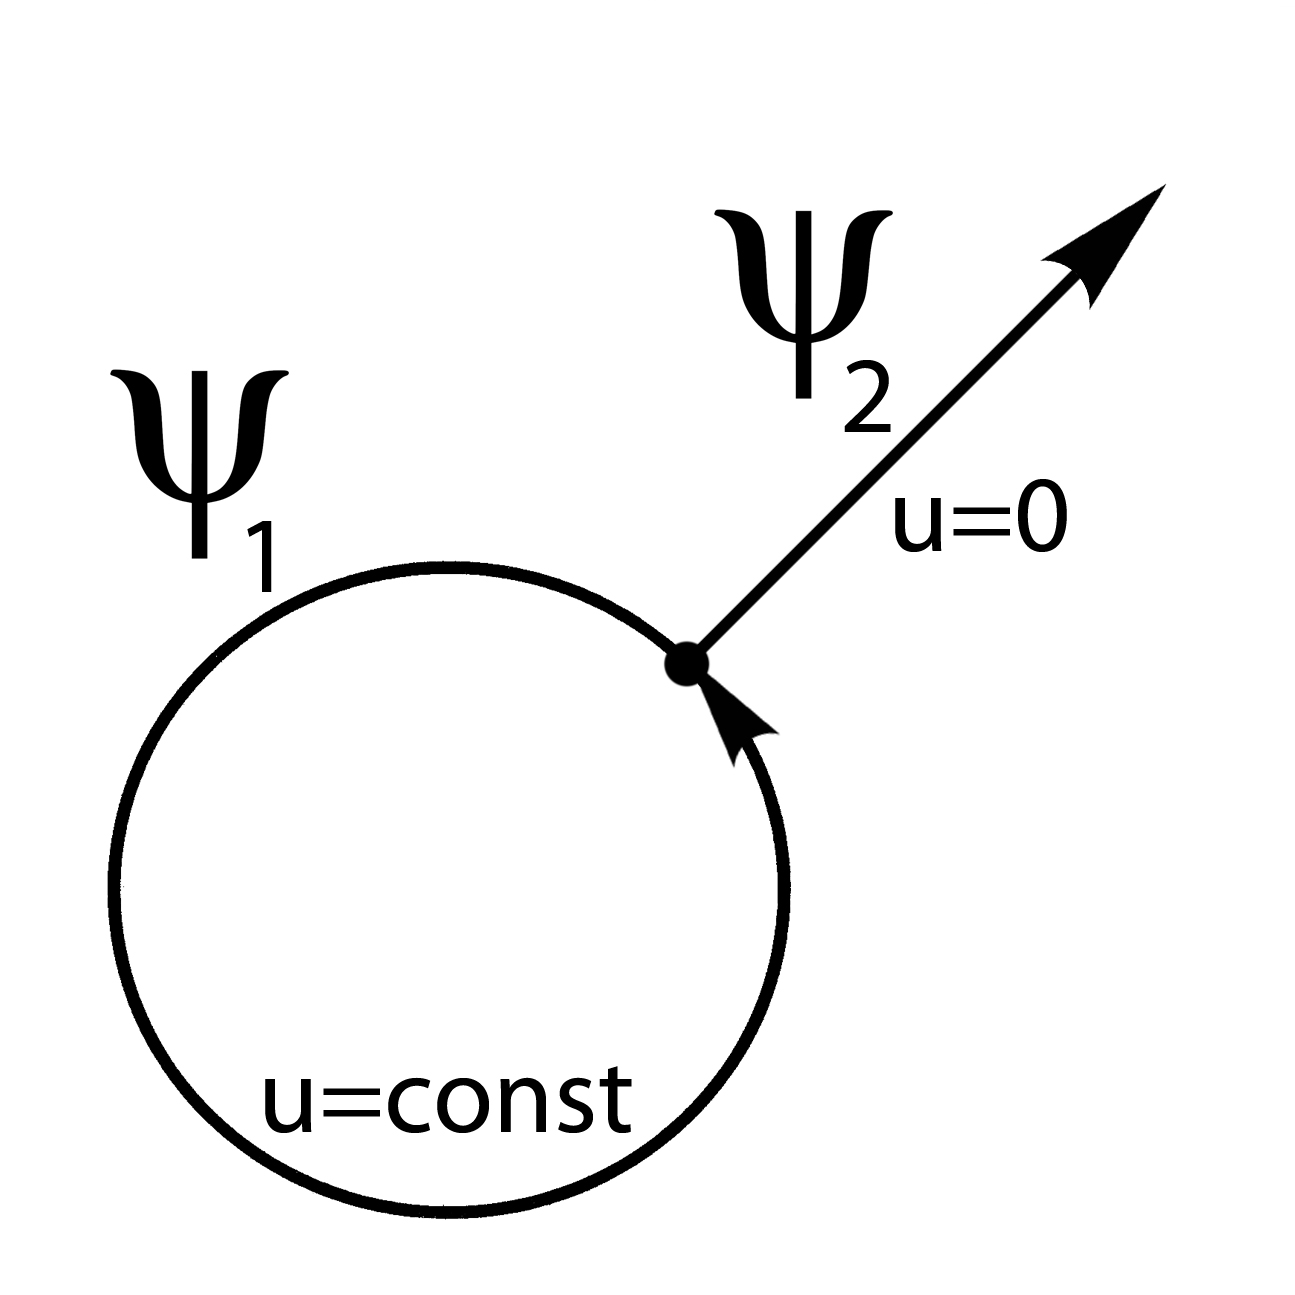
\includegraphics[scale=0.5]{one-arrow.jpg}
   \end{figure}


   Данные рассеяния для такого графа ~--- это коэффициент отражения $R$. Обозначив $p=\sqrt{u-k^2}$, запишем его в виде:
   \begin{equation}
   \label{OneDimensionalReflection}
   R\left(k,u\right) = {\frac { \left( ik+2\,p \right) {e}^{2\,pa}-ik-4\,p{e}^{pa}+2\,p}{ \left( ik-2\,p \right) {e}^{2\,pa}-ik+4\,p{e}^{pa}-2\,p}}
   \end{equation}
   
   Данное решение обладает интересным свойством: \[R\left(-k,u\right) = \frac{1}{R\left(k,u\right)} \ \forall k \in \mathbb{R}.\]
   
   Чтобы показать это, достаточно переписать коэффициент в виде
   \[ R\left(k,u\right) =
   \frac{-4p^2 \left(e^{pa}-1\right)^2 + k^2 \left(e^{pa}+1\right)^2}{4p^2 \left(e^{pa}-1\right)^2 + k^2 \left(e^{pa}+1\right)^2} + i \frac{-4pk\left(e^{2pa}-1\right)}{4p^2 \left(e^{pa}-1\right)^2 + k^2 \left(e^{pa}+1\right)^2}.\]
   Заметим, что $R\left(-k,u\right) = \overline{R\left(k,u\right)}$, тогда в силу унитарности $R$ получаем искомое свойство.  
   
   Как изменяются данные рассеяния при возмущениях константного потенциала?
   Чтобы понять это, рассмотрим поверхность, соответствующую вещественной части коэффициента отражения (\ref{OneDimensionalReflection}):
   
   \begin{figure}[!htb]
   	\begin{minipage}[h]{0.49\linewidth}
   		\center{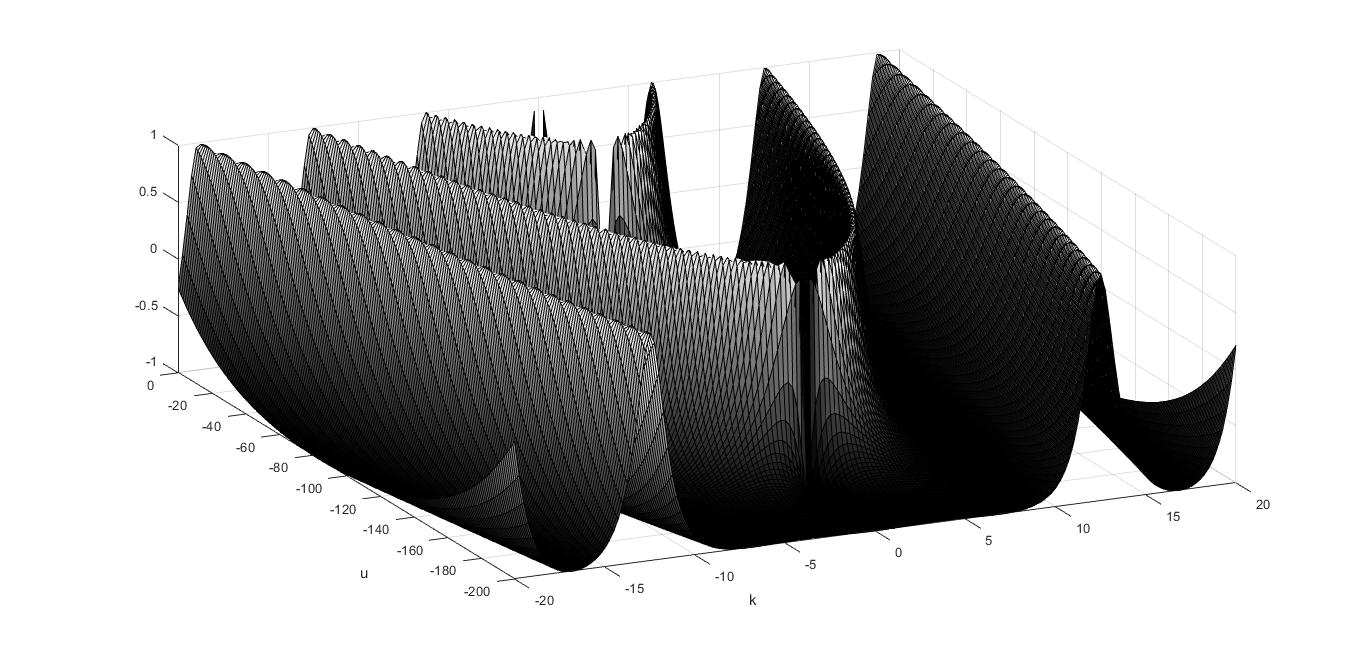
\includegraphics[width=\linewidth]{real_surface.jpg}}
   	\end{minipage}
      	\begin{minipage}[h]{0.49\linewidth}
   	\center{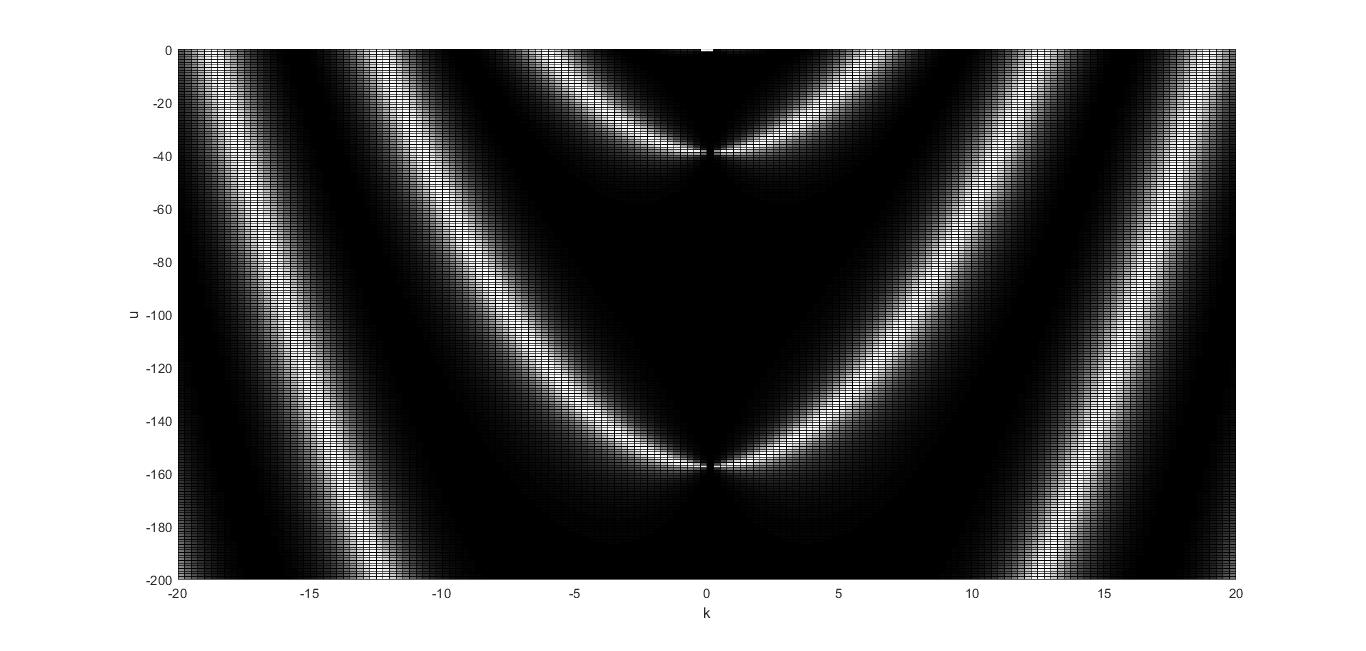
\includegraphics[width=\linewidth]{real_surface_top.jpg}}
   \end{minipage}
   \caption{Вещественная часть коэффициента отражения}
   \label{fig:real}
   \end{figure}
   
   \begin{figure}[!htb]
   \centering
   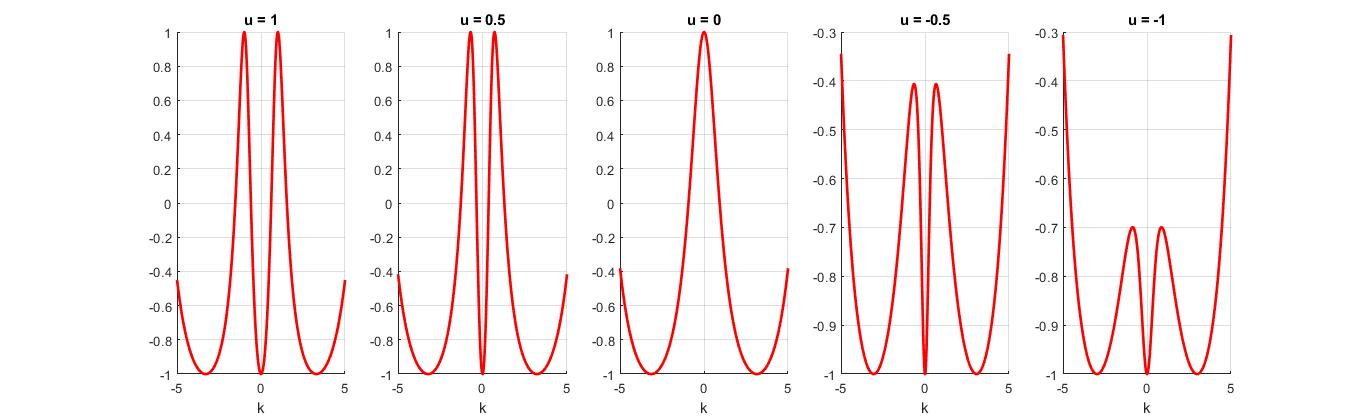
\includegraphics[scale=0.35]{real.jpg}
   \caption{Вещественная часть коэффициента отражения при различных значениях $u$}
   \end{figure}

   Из построений видно, что полученное решение напоминает набор параболических складок, гладко склеенных друг с другом. 
   При вариации константного потенциала на одном из рёбер рассматриваемого графа возникают ситуации, в которых сечение поверхности наталкивается на вершину новой параболы, что вызывает скачки искомого решения, а также препятствует сходимости данных рассеяния.
   Аналогичные наблюдения верны и для мнимой части коэффициента отражения:

   \begin{figure}[!htb]
   	\begin{minipage}[h]{0.49\linewidth}
   		\center{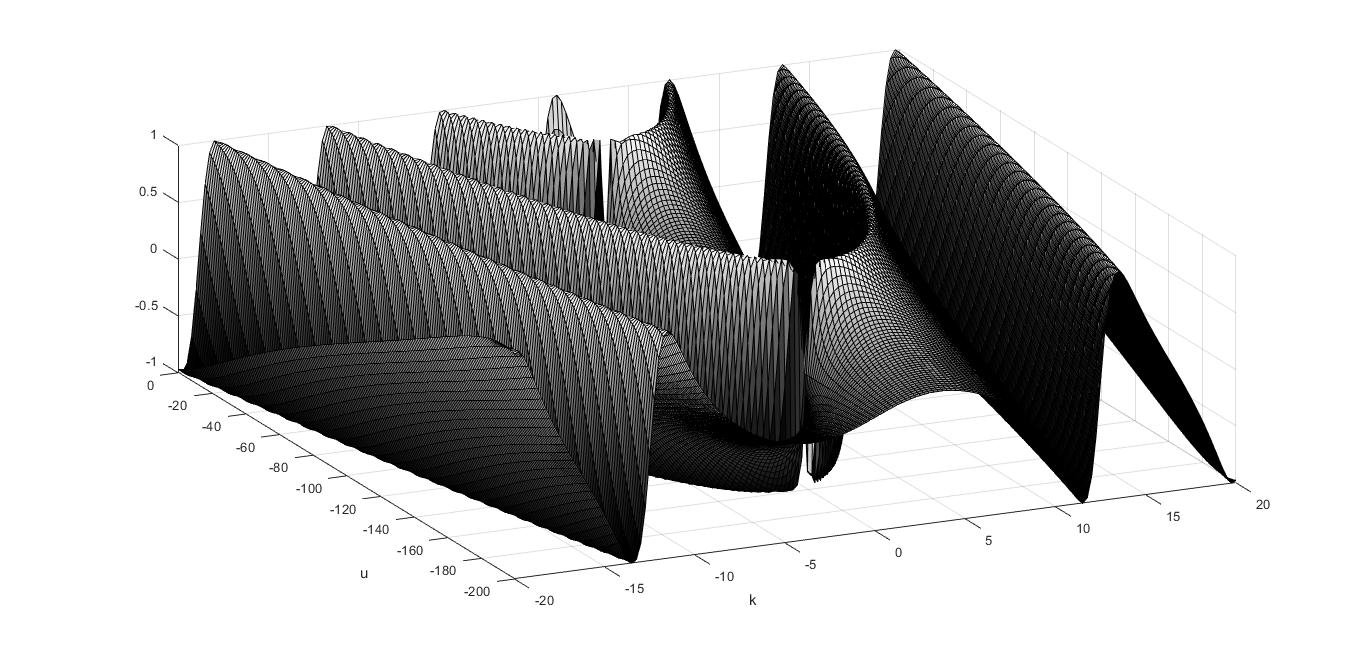
\includegraphics[width=\linewidth]{imag_surface.jpg}}
   	\end{minipage}
   	\begin{minipage}[h]{0.49\linewidth}
   		\center{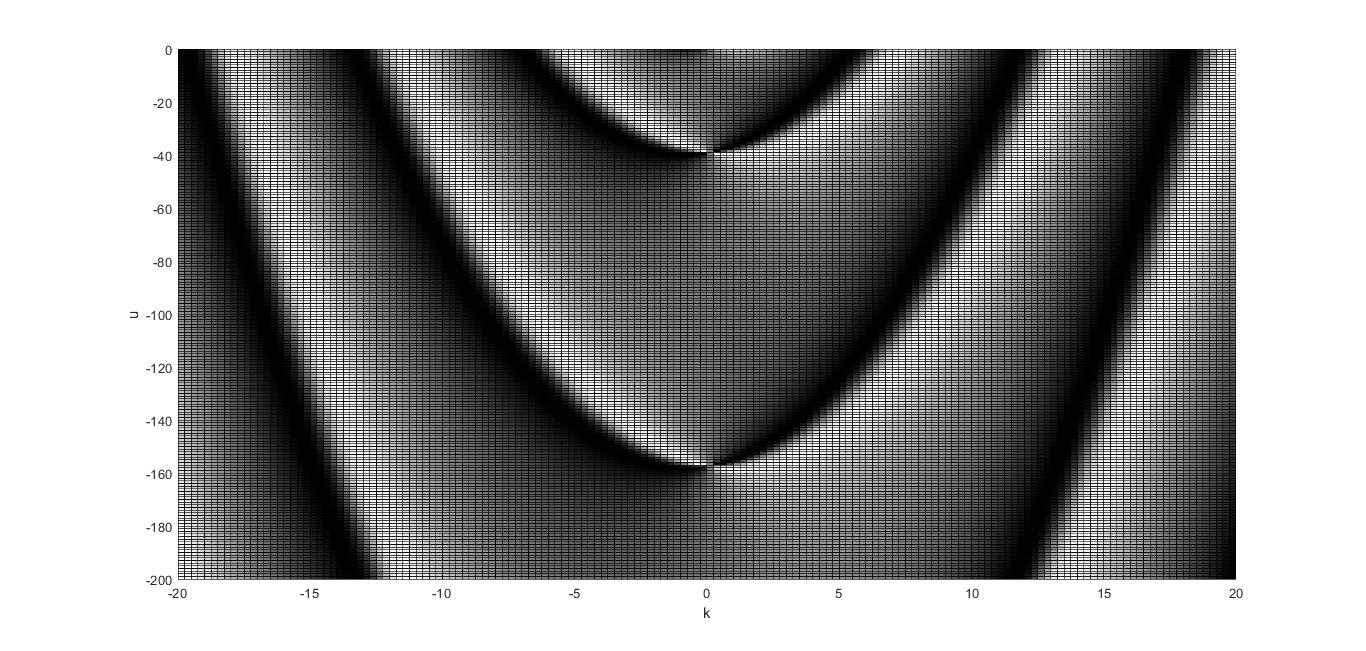
\includegraphics[width=\linewidth]{imag_surface_top.jpg}}
   	\end{minipage}
   	\caption{Мнимая часть коэффициента отражения}
   	\label{fig:imag}
   \end{figure}

   \begin{figure}[!htb]
   	\centering
   	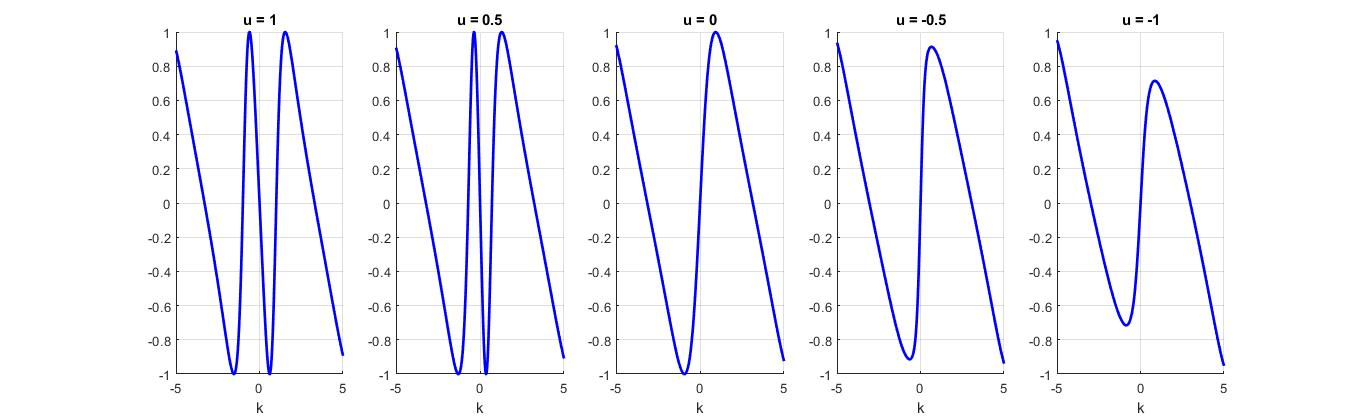
\includegraphics[scale=0.35]{imag.jpg}
   	\caption{Мнимая часть коэффициента отражения при различных значениях $u$}
   \end{figure}

   Причина скачков ~--- это особенности, являющиеся семейством вложенных друг в друга парабол. Получим их явный вид, определив нули знаменателя (\ref{OneDimensionalReflection}):
   
   \[\left( ik-2\,p \right) {e}^{2\,pa}-ik+4\,p{e}^{pa}-2\,p = 0 \longleftrightarrow \Re\left(\ldots\right) = 0, \Im\left(\ldots\right) = 0\]
   Следовательно, для вещественной части имеем:
   \begin{align*}
   -2pe^{2pa}+4pe^{pa}-2p &= 0 \\ e^{2pp} - 2e^{pa}+1 &= 0 \\
   \left(e^{pa}-1\right)^2 &= 0 \\
   e^{pa} &= 1 \\
   p &= \frac{2\pi n i}{a}, \ n \in \mathbb{Z}
   \end{align*}
   Для мнимой части коэффициента отражения имеем:
   \begin{align*}
   ke^{2pa} &=k \\
   e^{2pa} &= 1 \\
   p &= \frac{\pi n i}{a}
   \end{align*}
   Учитывая $p = \sqrt{u-k^2}$, получаем $\sqrt{u-k^2} = \frac{2\pi n i}{a}, n \in \mathbb{Z}$, и, как следствие,
   \[u = k^2 - \frac{4 \pi^2 n^2}{a^2}, \ n \in \mathbb{N}.
   \]
   
   Найденные особенности коэффициента отражения также присутствуют в решениях задачи рассеяния в графах-петлях и графах-кольцах с $n$ полубесконечными рёбрами.
   
   \subsection{МЕТОД МНОЖЕСТВЕННОГО РАССЕЯНИЯ}
   Исследовать полученные особенности помогает метод множественного рассеяния, описанный в \cite{Beam}. Этот метод основан на рассмотрении процесса рассеяния как последовательности отражений и прохождений.

   В качестве примера рассмотрим одномерную задачу рассеяния

   \begin{equation}\label{ScattPrBarr}
   -\frac{d^2\psi}{d x^2}+u\psi=k^2\psi,
   \end{equation}

   со ступенчатым потенциалом

   \begin{equation*}\label{BarrierPot}
   u(x)=\left\{%
   \begin{array}{ll}
   u_0, & |x|\leq a, \\
   0, & |x|>a \\
   \end{array}%
   \right.
   \end{equation*}

   Обозначив $K = \sqrt{u_0-k^2}$, полагая для определёности $u_0^2 > k^2$, будем искать решение такой задачи в виде:
   \[\begin{split}
   \psi_1\left(x\right) &= C_1 e^{ikx} + C_2 e^{-ikx}, \quad x\leq -a\\
   \psi_2\left(x\right) &= C_3 e^{Kx} + C_4 e^{-Kx}, \quad \left|x\right|\leq a\\
   \psi_3\left(x\right) &= C_5 e^{ikx} + C_6 e^{-ikx}, \quad x \geq a.
   \end{split}\]

   Предполагая, что волна падает на потенциальный барьер слева, перепишем решение в виде:

   \[\begin{split}
   \psi_1\left(x\right) &= e^{ikx} + R e^{-ikx}, \quad \ \ x\leq -a\\
   \psi_2\left(x\right) &= Ae^{Kx} + B e^{-Kx}, \quad \left|x\right|\leq a\\
   \psi_3\left(x\right) &= T e^{ikx}, \quad \quad \quad \quad \quad x \geq a.
   \end{split}\]

   Стандартный способ нахождения коэффициентов $A,\  B, \  R,\  T$  заключается в использовании непрерывности волновой функции, а также её производной в точках $a, \ -a$ \cite{Peisakhovich}.

   Решим эту задачу при помощи метода множественного рассеяния: рассмотрим преломление волны в точке $-a$, затем проследуем за прошедшей через барьер волной до точки $a$. В этой точке волна снова преломляется: одна часть выходит из барьера, в то время как оставшаяся часть двигается в отрицательном направлении до точки $-a$, где процесс аналогично продолжается до бесконечности. Таким образом, коэффициенты отражения и прохождения ~--- это суммы многократно отражённых и прошедших волн. Таким же способом можно вычислить решение на отрезке $\left|x\right|\leq a$.

   Рассмотрим первое преломление падающей слева волны в точке $-a$:
   
   \begin{figure}[!htb]
   	\centering
   	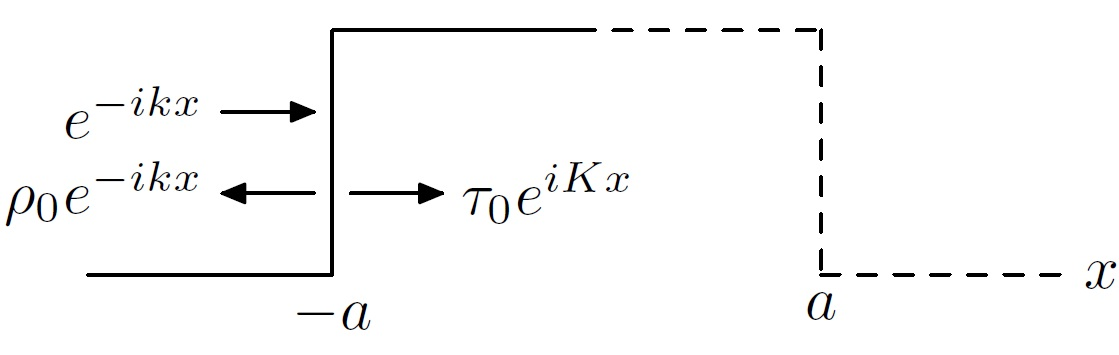
\includegraphics[scale=0.25]{reflect1.jpg}
   	\caption{Первое преломление падающей слева волны}
   \end{figure}

   В таком случае волновая функция примет вид:
   
   \begin{equation*}
   \psi(x)=\left\{%
   \begin{array}{ll}
   e^{ikx}+\rho_0e^{-ikx} & x<-a, \\
   \tau_0 e^{iKx} & x>-a. \\
   \end{array}%
   \right.
   \end{equation*}

   Пользуясь непрерывностью волновой функции и её производной, определим $\rho_0, \ \tau_0$:

   \[
   \begin{aligned}
   \rho_0&=\frac{k-K}{k+K}e^{-2ika},\\
   \tau_0&=\frac{2k}{k+K}e^{-i(k-K)a}.
   \end{aligned}\]
   
   Рассмотрим волну, которая прошла через границу потенциального барьера и сталкивается с правой границей:
   
   \begin{figure}[!htb]
   	\centering
   	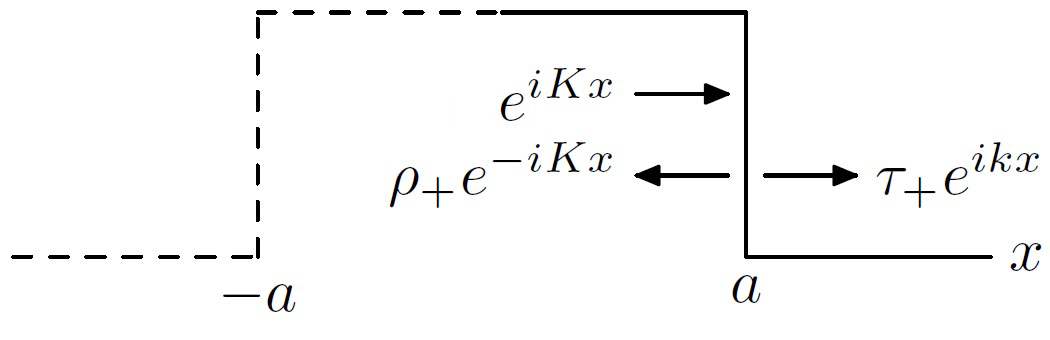
\includegraphics[scale=0.25]{reflect2.jpg}
   	\caption{Второе преломление падающей слева волны}
   \end{figure}

   В таком случае волновая функция примет вид:
   
   \[
   \psi(x)=\left\{%
   \begin{array}{ll}
   e^{iKx}+\rho_+e^{-iKx} & x<a, \\
   \tau_+e^{ikx} & x>a. \\
   \end{array}%
   \right.
   \]
   
   Используя непрерывность, получим:
   
   \[
   \begin{aligned}
   \rho_+&=-\frac{k-K}{k+K}e^{2iKa},\\
   \tau_+&=\frac{2K}{k+K}e^{-i(k-K)a}.
   \end{aligned}
   \]
   
   Рассмотрим преломление волны, которая была отражена от правой границы, и достигла левой границы:
   
   \begin{figure}[!htb]
   	\centering
   	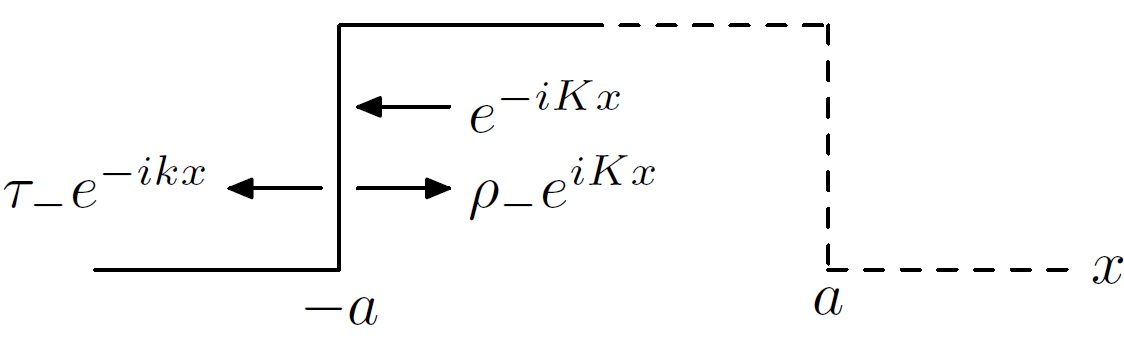
\includegraphics[scale=0.25]{reflect3.jpg}
   	\caption{Преломление отражённой от правой границы волны на левой границе}
   \end{figure}

   В таком случае волновая функция имеет вид:
   
   \[
   \psi(x)=\left\{%
   \begin{array}{ll}
   e^{-iKx}+\rho_-e^{-iKx} & x>-a, \\
   \tau_-e^{-ikx} & x<-a, \\
   \end{array}%
   \right.
   \]
   
   Коэффициенты $\rho_-, \tau_-$ в силу симметрии совпадают с коэффициентами $\rho_+, \tau_+$ соответственно. Обозначим $\rho = \rho_- = \rho_+, \ \tau = \tau_- = \tau_+$.
   
   \pagebreak
   Рассматривая бесконечный процесс рассеяния,
   
   \begin{figure}[!htb]
   	\centering
   	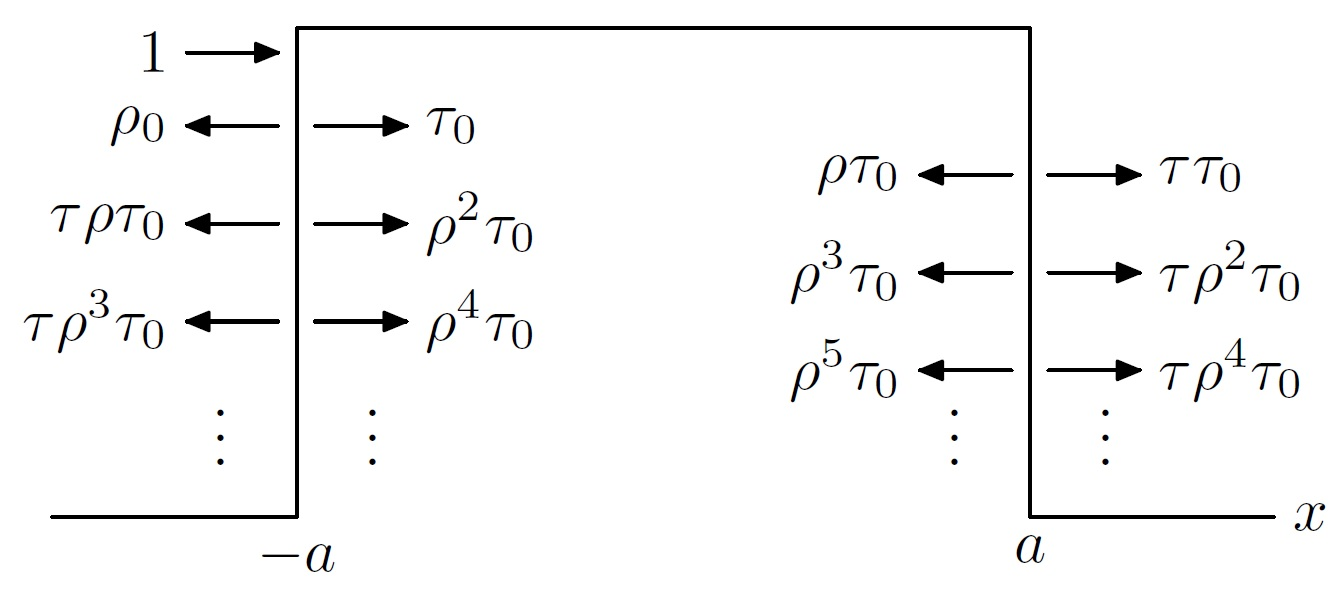
\includegraphics[scale=0.25]{reflect4.jpg}
   	\caption{Амплитуды волн при множественном рассеянии}
   \end{figure}

   и суммируя амплитуды волн, получим следующие выражения для коэффициентов отражения и прохождения:
   
   \[
   \begin{aligned}
   R&=\rho_0+\tau(\rho+\rho^3+\rho^5+\ldots)\tau_0=\rho_0+\frac{\tau\rho\tau_0}{1-\rho^2},\\
   T&=\tau(1+\rho^2+\rho^4+\ldots)\tau_0=\frac{\tau\tau_0}{1-\rho^2}, \\
   A&=(1+\rho^2+\rho^4+\ldots)\tau_0=\frac{\tau_0}{1-\rho^2}, \\
   B&=(\rho+\rho^3+\rho^5+\ldots)\tau_0=\frac{\rho\tau_0}{1-\rho^2}.   
   \end{aligned}\]
   
   Нетрудно заметить, что $|\rho|<1$, поэтому полученные ряды сходятся.   
   
   Аналогичные идеи можно применить и для рассеяния на графах.
   
   \subsubsection{ГРАФ-ПЕТЛЯ С 1 ПОЛУБЕСКОНЕЧНОЙ ДУГОЙ И НУЛЕВЫМ ПОТЕНЦИАЛОМ НА ПЕТЛЕ}
   
   Рассмотрим рассеяние свободной частицы на графе-петле длины $a$, содержащем одну полубесконечную дугу:
   
   \begin{figure}[!htb]
   	\centering
   	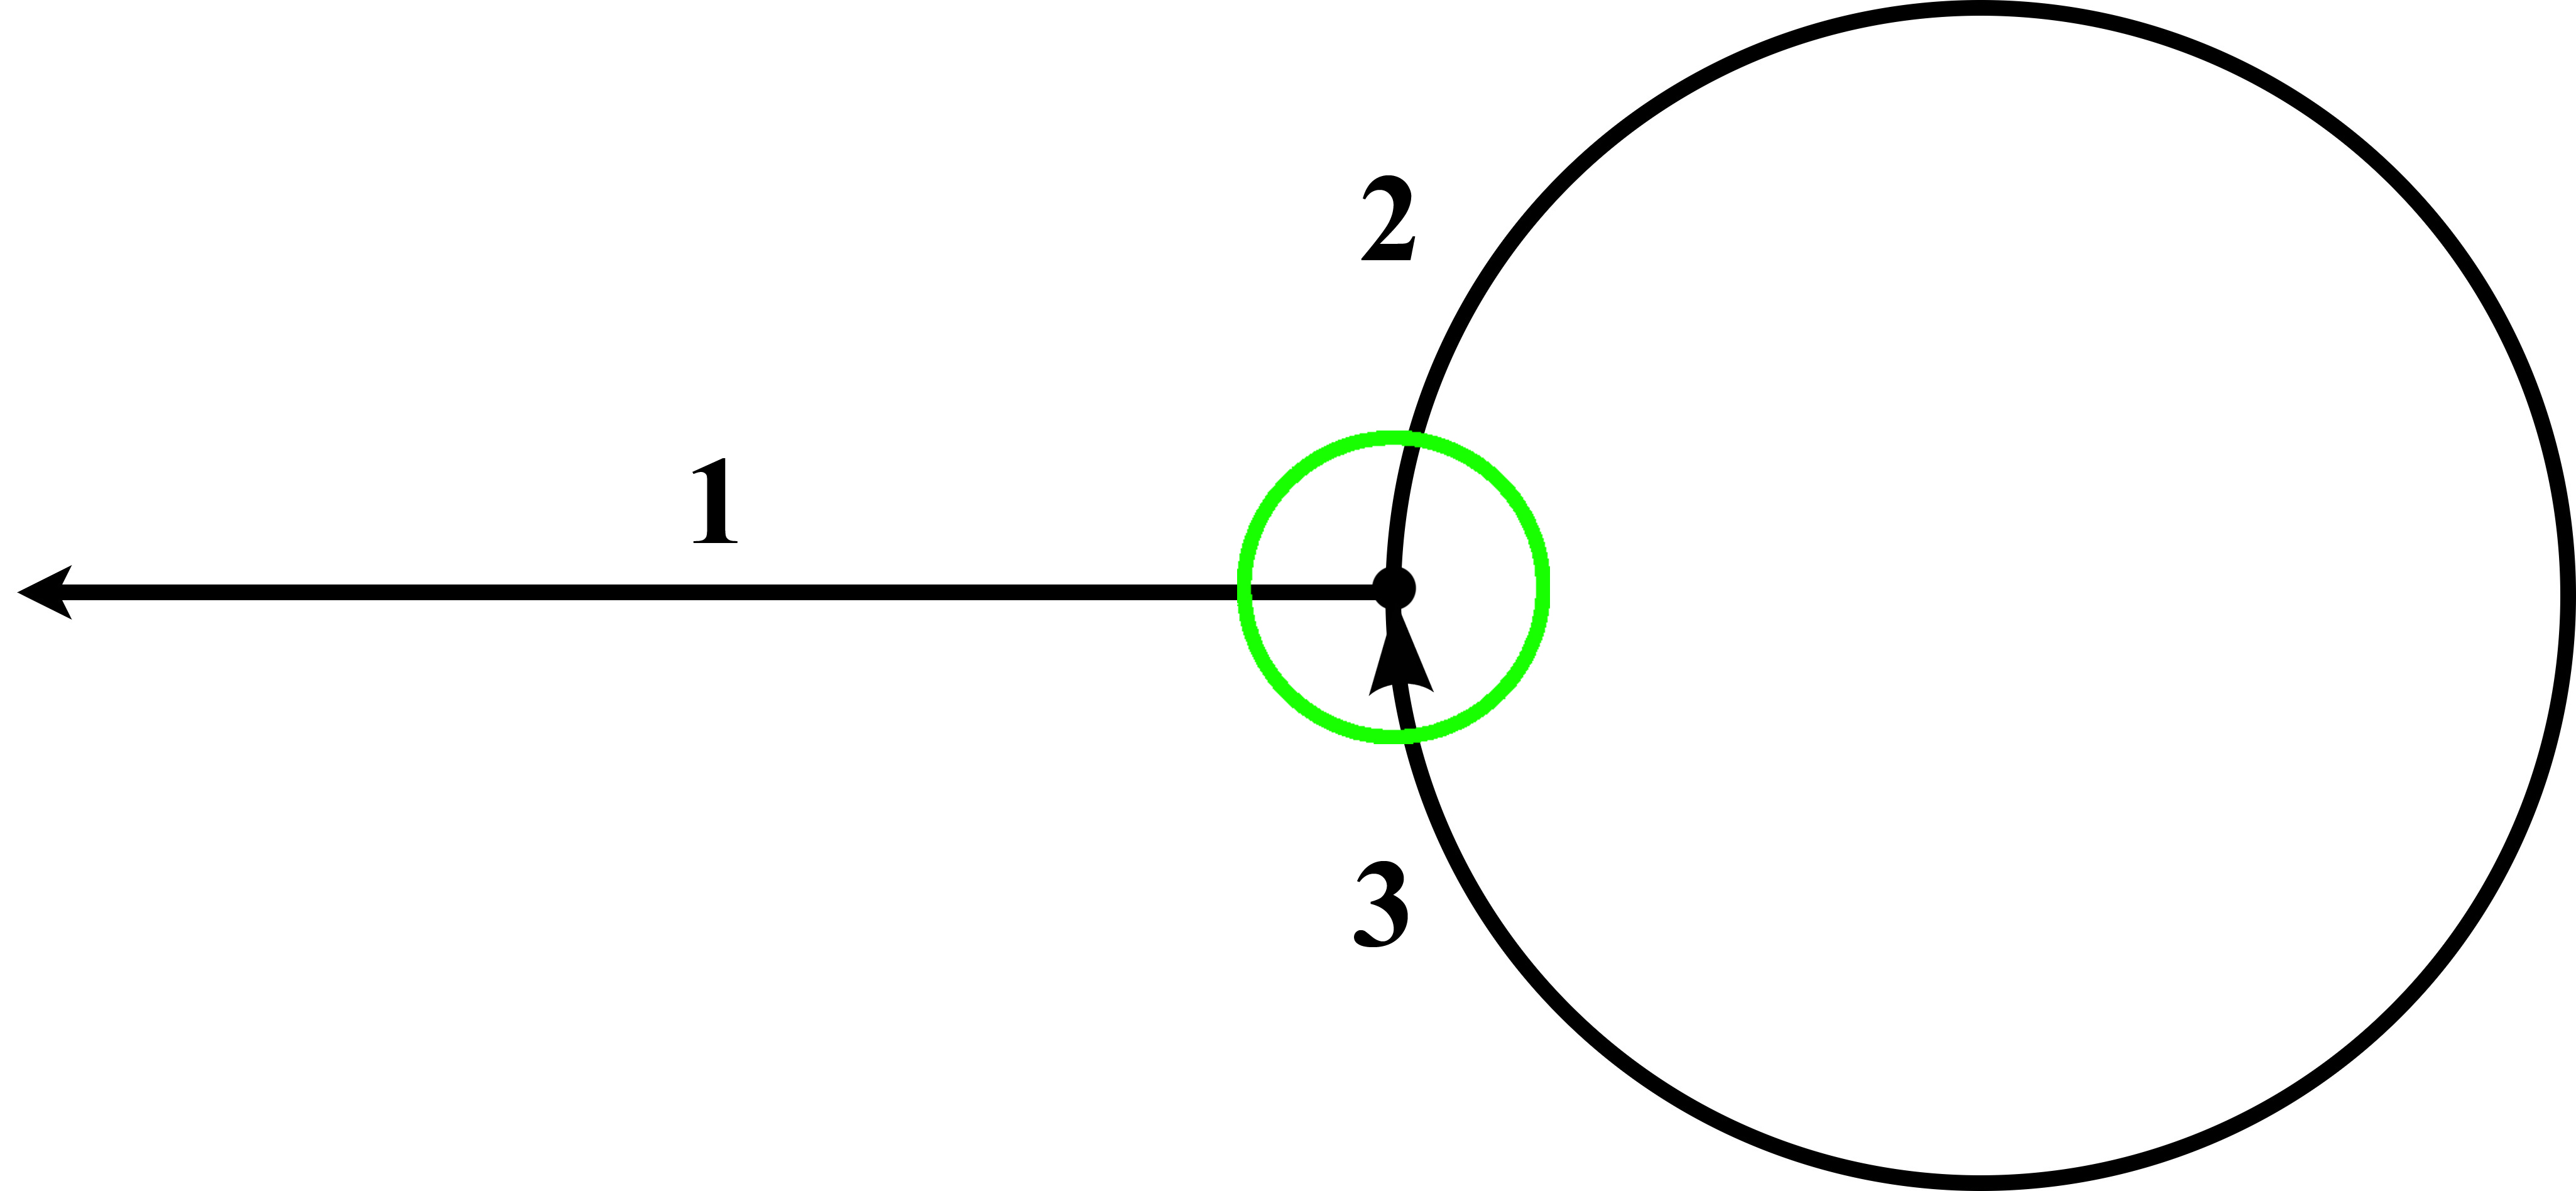
\includegraphics[scale=0.05]{circle1.jpg}
    \caption{Граф-петля с 1 полубесконечной дугой, вершина окружена окрестностью малого радиуса}
   \end{figure}
   
   Зная общий вид решения и используя законы Кирхгофа, можно получить следующее соотношение для коэффициента отражения:
   \begin{equation}
   \label{multiplyReflection1}
   R = \frac{1-3e^{ika}}{e^{ika}-3}
   \end{equation}
   
   Очень удобным инструментом для исследования рассеяния на графах является преобразование Фурье по спектральному параметру.
   Можно заметить, что \[  R = \frac{1-3e^{ika}}{e^{ika}-3} = -\frac{1}{3} + 8 \sum_{n=1}^{+\infty}\frac{1}{3^{n+1}}e^{ikan},\]
   
   Имея представление коэффициента отражения (\ref{multiplyReflection1}) в виде ряда по экспонентам, можно легко посчитать преобразование Фурье:
   \[\widehat{R}(\omega)=-\frac{2\pi}{3}\delta(\omega)+16\pi\sum_{n=1}^{\infty}\frac{1}{3^{n+1}}\delta(\omega-na).\]
   
   Здесь $\delta\left(\omega -na\right)$ ~--- запаздывающая $\delta$-волна, прошедшая по петле $n$ раз, а затем вышедшая по полубесконечной дуге. Коэффициент при $\delta$-функции ~--- амплитуда, умноженная на $2\pi$.
   
   Рассматривая это представление, можно заметить, что слагаемое перед основной суммой состоит из волны, которая отразилась от вершины графа и ни разу не прошла по петле. Слагаемое, соответствующее $n=k$, соответствует сумме волн, которые прошли по петле ровно $k$ раз, а затем покинули граф по полубесконечной дуге.
   
   Полученные выкладки использовали известный «метод тщательного разглядывания», что несколько усложняет аналогичные выкладки для графов с ненулевым значением потенциалов.
   
   Разложение коэффициента отражения (\ref{multiplyReflection1}) можно получить методом множественного рассеяния. В таком случае верна формула:
   
   \begin{equation}
   \label{multiple}
   R\left(k,u\right) = \sum_{\text{по путям длины $a \cdot n$}} e^{ikan} \cdot a\left(n\right).
   \end{equation}
   
   Рассмотрим поведение коэффициента $a\left(n\right)$:
   \[\begin{aligned}
   a(0) &= -\frac{1}{3} \\
   a(1) &= \frac{4}{9} + \frac{4}{9} = \frac{8}{9} \\
   a(2) &= \frac{8}{27} - \frac{4}{27} + \frac{8}{27} - \frac{4}{27} =  \frac{8}{27}
   \end{aligned}\]
   
   В данном случае преломление волн происходит только в вершине графа, поэтому можно окружить вершину окружностью малого радиуса (см. Рис. 9) и решить задачу рассеяния для графа-звезды с тремя полубесконечными дугами и нулевыми потенциалами. Напомним данные рассеяния для такой задачи (\ref{starData}):
   
   \[
   S(k)=
   \begin{pmatrix}
   -1/3 & 2/3 & 2/3 \\
   2/3 & -1/3 & 2/3 \\
   2/3 & 2/3 & -1/3 
   \end{pmatrix}\]
   
   Процесс множественного рассеяния можно описать в терминах данных рассеяния:
   
   \[
   \begin{aligned}
   a(0) &= R_{11} \\
   a(1) &= T_{12}\cdot T_{31} + T_{13}\cdot T_{21} \\
   a(2) &= T_{12}\cdot T_{32}\cdot T_{31} + T_{12} \cdot R_{33} \cdot T_{21} + T_{13} \cdot T_{23} \cdot T_{21} + T_{13} \cdot R_{22} \cdot T_{31}
   \end{aligned}\]
   
   \subsubsection{ГРАФ-ПЕТЛЯ С 1 ПОЛУБЕСКОНЕЧНОЙ ДУГОЙ И КОНСТАНТНЫМ ПОТЕНЦИАЛОМ НА ПЕТЛЕ}
   
   To be continued....
   
   
   \newpage
   \section{ЗАКЛЮЧЕНИЕ}
   
   В данной работе было рассмотрено несколько задач: задача склейки графов по двум рёбрам, а также задача исследования сходимости данных рассеяния при константных возмущениях потенциалов.
   
   Были получены теоремы о склейке графов, имеющих 3 полубесконечных дуги с нулевыми потенциалами, неизвестную компактную часть по двум рёбрам в ребро единичной длины. 
   
   Для исследования сходимости были получены решения для некоторых частных случаев графов (петли и кольца с $n$ полубесконечными дугами, звёздные графы) и потенциалов на внутренних рёбрах. Были исследованы свойства данных рассеяния для таких графов, численно изучены эффекты возникновения возмущений при константных трансформациях потенциала, а также предложен способ дальнейшего исследования задачи.

  
   
   
\newpage.
\addcontentsline{toc}{section}{ЛИТЕРАТУРА}
\renewcommand{\refname}{ЛИТЕРАТУРА}
\begin{thebibliography}{1} % Ссылки на литературу приводятся только на английском языке (даже если у источника нет англоязычной версии).
	
	\bibitem{TransparentQuantumGraphs} J.~R.~Yusupov, K.~K.~Sabirov, M.~Ehrhardt, D.~U.~Matrasulov, {\it Transparent Quantum Graphs}, Phys. Lett. A 383, 2382 (2019).
	
	\bibitem{KirchhoffRule} V.~Kostrykin, R.~Schrader, {\it Kirchhoff's Rule for Quantum Wires} J. Phys. A: Math. Gen. Vol.32, (1999), 595--630.
	
	\bibitem{Kuhn} H.~Kuhn, {\it A Quantum-Mechanical Theory of Light Absorption of Organic Dyes and Similar Compounds}, J. Chem. Phys. \textbf{17} (1949), https://doi.org/10.1063/1.1747143.
	
	\bibitem{Superconductivity} S.~Alexander, {\it Superconductivity of networks. A percolation approach to the effects of disorder}, Phys. Rev. B \textbf{27}, 1541 (1983).
	
	\bibitem{Kowal} D.~Kowal, U.~Sivan, O.~Entin-Wohlman, Y.~Imry, {\it Transmission through multiply-connected wire systems}, Phys. Rev. B \textbf{42}, 9009 (1990).

	\bibitem{QuantumChaos} T.~Kottos, U.~Smilansky, {\it Quantum chaos on graphs}, Phys. Rev. Lett. \textbf{79}, 4794--7 (1997).
	
	\bibitem{SpectralEstimates} A.~Kostenko, N.~Nicolussi, {\it Spectral estimates for infinite quantum graphs}, Calc. Var. \textbf{58}, 15 (2019), Spectral estimates for infinite quantum graphs.
	
	\bibitem{deltaCouplings}  P.~Kurasov, A.~Serio, {\it Optimal Potentials for Quantum Graphs}, Ann. Henri Poincare \textbf{20}, 1517--1542 (2019). https://doi.org/10.1007/s00023-019-00783-6
	
	\bibitem{Popov1} D.~A.~Eremin, E.~N.~Grishanov, D.~S.~Nikiforov, I.~Y.~Popov, {\it Wave dynamics on time-depending graph with Aharonov-Bohm ring}, Наносистемы: физика, химия, математика, \textbf{9}:4 (2018), 457--463. https://doi.org/10.17586/2220-8054-2018-9-4-457-463
	
	\bibitem{Popov2} A.~A.~Boitsev, I.~Y.~Popov, {\it A model of an electron in a quantum graph interacting with a two-level system}, Наносистемы: физика, химия, математика, \textbf{10}:2 (2019), 131--140. https://doi.org/10.17586/2220-8054-2019-10-2-131-140
	
	\bibitem{GerasimenkoPavlov} Н.~И.~Герасименко, Б.~С.~Павлов, {\it Задача рассеяния на некомпактных графах}, ТМФ, \textbf{74}:3 (1988), 345 -- 359.
	
	\bibitem{SpectralSurgery} А.~Н.~Бондаренко, В.~А.~Дедок, {\it Спектральная хирургия квантовых графов}, Сиб. журн. индустр. матем., \textbf{7}:4 (2004), 16--28.
	
	\bibitem{Peisakhovich} Ю.~Г.~Пейсахович, А.~А.~Штыгашевич, {\it Одномерная квантовая механика}, монография, Новосибирск, Изд-во НГТУ, 2007.
	
	\bibitem{Landau} Л.~Д.~Ландау, Е.~М.~Лифшиц, {\it Квантовая механика (нерелятивистская теория)}, Издание 4-е, М.:Наука 1989, 768 с. - (<<Теоретическая физика>>, том \RomanNumeralCaps{3}) - ISBN 5-02-014421-5.
	
	\bibitem{SMatrix} Л.~Д.~Фаддеев, {\it Свойства $S$-матрицы одномерного уравнения Шрёдингера}, Труды МИАН, 1964, Т.73, с. 314--336.
	
	\bibitem{Kolmogorov} А.~Н.~Колмогоров, С.~В.~Фомин, {\it Элементы теории функций и функционального анализа}, 4-е изд., М.:Наука, 1976, 544 с.
	
	\bibitem{Beam} J.~E.~Beam, {\it Multiple Reflection in Potential-Barrier Scattering}, Am. J. Phys \textbf{38}, pp. 1395--1401, 1970.
	
	
	
\end{thebibliography}
\end{document}
